% !TEX root = ../do-an.tex
% =====================================================================
%  CHƯƠNG 2 — THỰC NGHIỆM
% =====================================================================
\chapter{Thực nghiệm}
\label{ch:thuc-nghiem}

\begin{muctieu}
Chương này trình bày toàn diện các kết quả thực nghiệm đạt được từ Bài nhận thức 2 đến Bài nhận thức 5: phân tích 4 sơ đồ tuần tự chuẩn UML, giải thuật lập lịch mạng PERT/CPM và tính toán đường găng, thực nghiệm quy trình thiết kế giao diện từ Wireframe đến ứng dụng thực tế, cùng thiết kế cơ sở dữ liệu và các tập dữ liệu thử nghiệm.
\end{muctieu}

\section{Sơ đồ tuần tự (Sequence Diagram) \& Sơ đồ luồng (Flowchart)}
\label{sec:sequence-diagram}

Sơ đồ tuần tự (Sequence Diagram) là biểu đồ tương tác thuộc chuẩn UML 2.5, mô hình hóa trình tự thời gian của các thông điệp trao đổi giữa các đối tượng để hoàn thành một ca sử dụng (Use Case) cụ thể. Cấu trúc mỗi sơ đồ gồm 4 thành phần quy chuẩn:
\begin{itemize}
    \item \textbf{Tác nhân (Actor):} Đại diện cho người dùng trực tiếp thao tác (Khách hàng đặt sân hoặc Chủ sân / Nhân viên bốt trực).
    \item \textbf{Lớp giao diện (Boundary):} Đại diện cho màn hình ứng dụng di động React Native tiếp nhận tương tác chạm và hiển thị dữ liệu.
    \item \textbf{Lớp điều khiển (Controller):} Đại diện cho tầng xử lý logic nghiệp vụ máy chủ Node.js/Express.
    \item \textbf{Lớp thực thể (Entity / Database):} Đại diện cho hệ cơ sở dữ liệu quan hệ MySQL lưu trữ bền vững các bảng quan hệ.
\end{itemize}
Song song với mô hình tương tác hướng đối tượng, sơ đồ luồng quy trình nghiệp vụ (Flowchart) thể hiện tiến trình điều khiển logic tuần tự từ điểm khởi đầu (Start), qua các khối xử lý và các nút rẽ nhánh điều kiện (Decision Points), đến khi kết thúc (End).

\subsection{Sơ đồ tuần tự và Sơ đồ luồng chức năng Đăng ký}
\textbf{a. Sơ đồ tuần tự chức năng Đăng ký tài khoản:}

\textbf{Tác nhân tham gia:} Khách hàng mới (Customer), Giao diện đăng ký (\code{RegisterScreen}), Bộ điều khiển xác thực (\code{AuthController}) và Bảng dữ liệu người dùng (\code{Users Table}).

\textbf{Mô tả luồng xử lý tuần tự:} Khách hàng nhập thông tin gồm Họ tên, Số điện thoại (10 chữ số), Email và Mật khẩu. Giao diện thực hiện kiểm tra tính hợp lệ cơ bản tại máy khách (Client-side validation) rồi gửi yêu cầu HTTP POST \code{/api/auth/register} đến máy chủ. Controller kiểm tra sự tồn tại của số điện thoại và email trong CSDL MySQL. Nếu dữ liệu hợp lệ và chưa từng được đăng ký, máy chủ tiến hành băm mật khẩu bảo mật (Bcrypt), khởi tạo bản ghi mới với vai trò \code{customer}, lưu xuống MySQL và trả về thông báo tạo tài khoản thành công kèm điều hướng về màn hình Đăng nhập.

\begin{figure}[H]
\centering
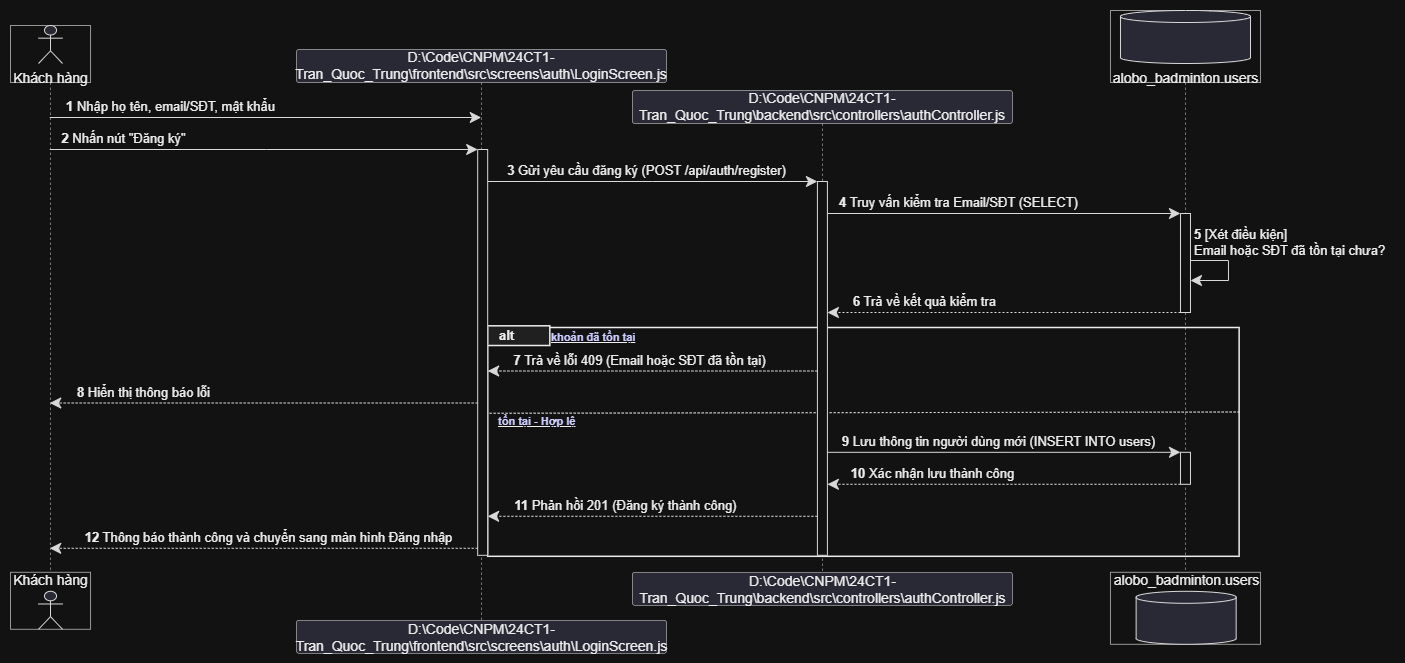
\includegraphics[width=0.88\textwidth]{figs/seq_dangky.png}
\caption{Sơ đồ tuần tự (Sequence Diagram) chức năng Đăng ký tài khoản người dùng.}
\label{fig:seq-dangky}
\end{figure}

\textbf{b. Sơ đồ luồng nghiệp vụ chức năng Đăng ký tài khoản:}

\textbf{Mô tả luồng nghiệp vụ:} Người dùng mở ứng dụng và chuyển sang màn hình Đăng ký tài khoản $\rightarrow$ Người dùng điền Họ tên, Số điện thoại (bắt buộc), Địa chỉ Email (kiểm tra định dạng hợp lệ) và Mật khẩu (tối thiểu 6 ký tự) $\rightarrow$ Khi nhấn "Đăng ký", hệ thống kiểm tra tính hợp lệ dữ liệu $\rightarrow$ Kiểm tra trùng lặp tài khoản trên CSDL: nếu đã tồn tại thì báo lỗi 409 Conflict $\rightarrow$ Nếu hợp lệ thì lưu người dùng mới vào MySQL và tự động chuyển về trang Đăng nhập.

\begin{figure}[H]
\centering
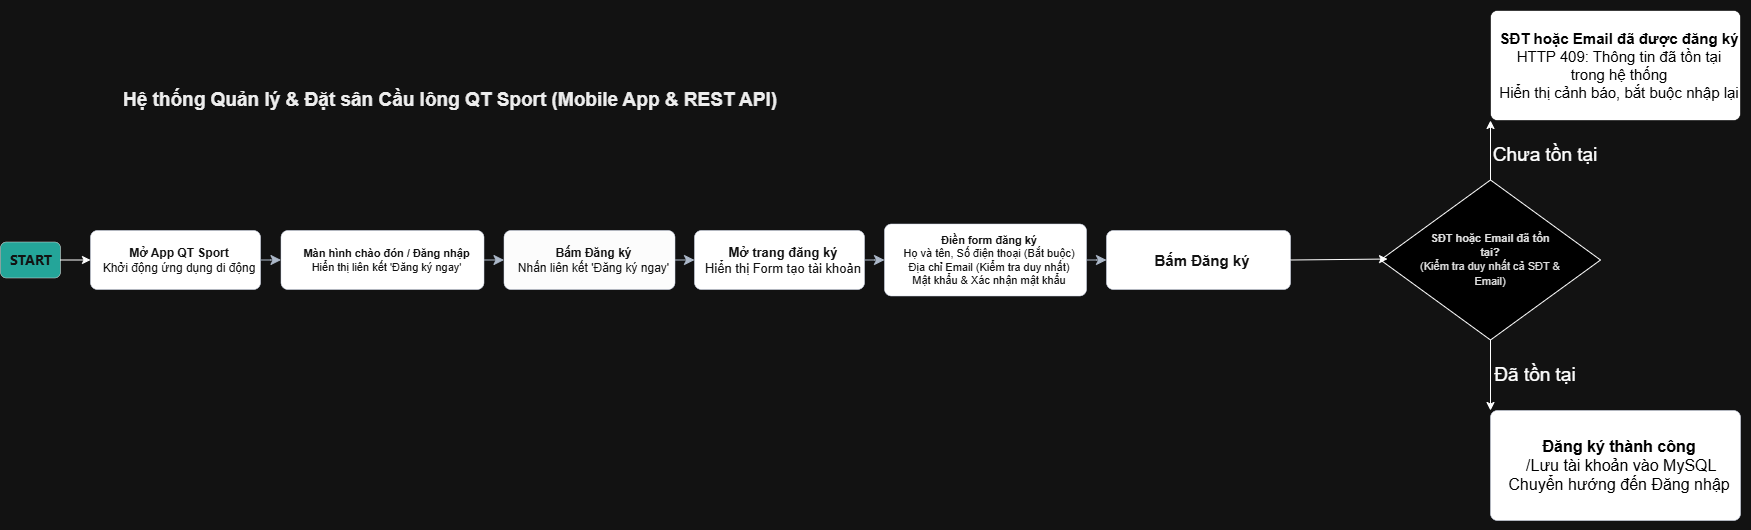
\includegraphics[width=0.88\textwidth]{figs/luong_dangky.png}
\caption{Sơ đồ luồng (Flowchart) chức năng Đăng ký tài khoản.}
\label{fig:luong-dangky}
\end{figure}

\newpage

\subsection{Sơ đồ tuần tự và Sơ đồ luồng chức năng Đăng nhập}
\textbf{a. Sơ đồ tuần tự chức năng Đăng nhập hệ thống:}

\textbf{Tác nhân tham gia:} Người dùng (User), Màn hình đăng nhập (\code{LoginScreen}), Bộ điều khiển xác thực (\code{AuthController}) và Bảng dữ liệu người dùng (\code{Users Table}).

\textbf{Mô tả luồng xử lý tuần tự:} Người dùng nhập Số điện thoại hoặc Email cùng Mật khẩu. Giao diện gửi yêu cầu HTTP POST \code{/api/auth/login} đến máy chủ. Controller truy vấn CSDL để tìm kiếm người dùng theo định danh tài khoản. Nếu tìm thấy và mật khẩu khớp với chuỗi băm lưu trữ, hệ thống khởi tạo chuỗi mã thông báo JSON Web Token (JWT) có hiệu lực 7 ngày chứa thông tin định danh và phân quyền vai trò (Role: \code{admin}, \code{staff} hoặc \code{customer}). Phía ứng dụng di động lưu JWT vào bộ nhớ bảo mật và Context API, tự động điều hướng người dùng đến giao diện tương ứng theo quyền hạn.

\begin{figure}[H]
\centering
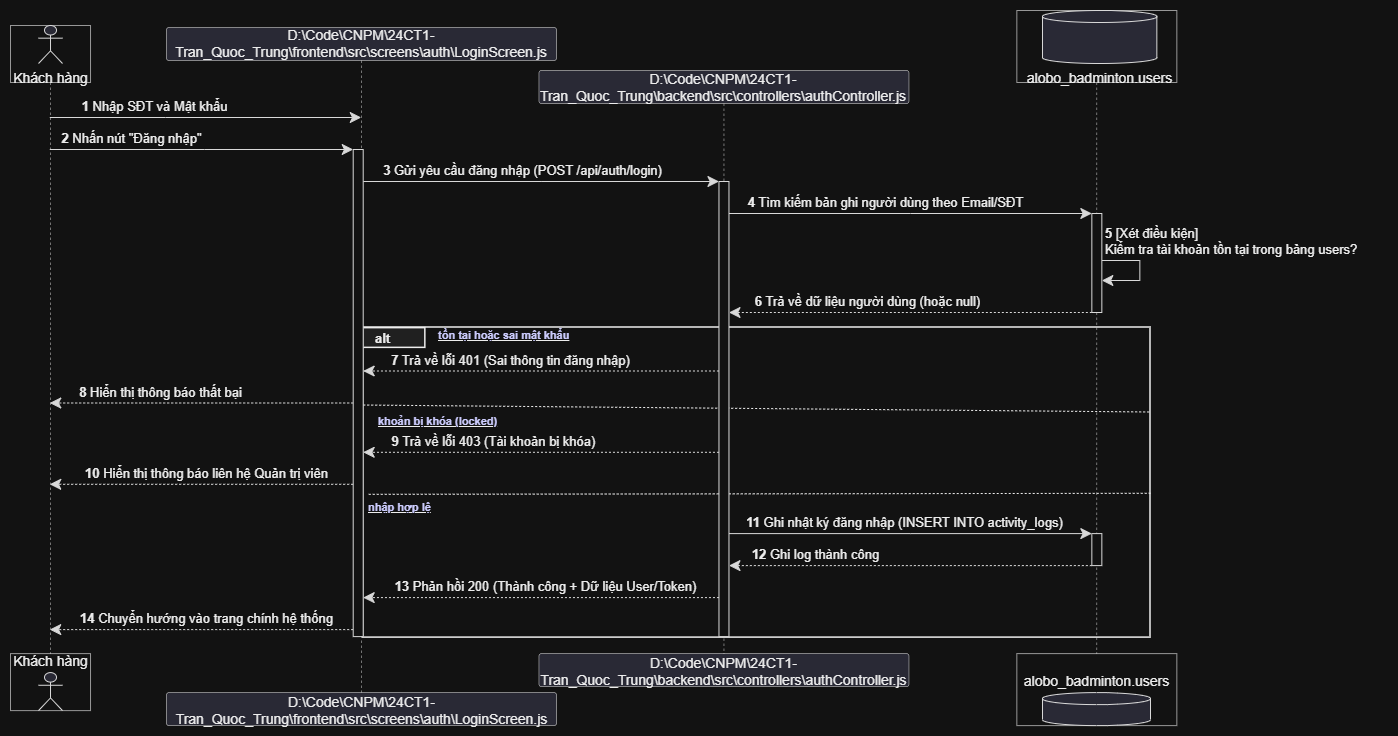
\includegraphics[width=0.88\textwidth]{figs/seq_dangnhap.png}
\caption{Sơ đồ tuần tự (Sequence Diagram) chức năng Đăng nhập hệ thống đa vai trò.}
\label{fig:seq-dangnhap}
\end{figure}

\textbf{b. Sơ đồ luồng nghiệp vụ chức năng Đăng nhập hệ thống:}

\textbf{Mô tả luồng nghiệp vụ:} Người dùng mở ứng dụng và tại màn hình đăng nhập thực hiện điền Số điện thoại/Email và Mật khẩu $\rightarrow$ Sau khi bấm "Đăng nhập", hệ thống gửi yêu cầu xác thực $\rightarrow$ Nếu thông tin không chính xác hoặc tài khoản không tồn tại, trả về lỗi 401; trường hợp tài khoản bị khóa, trả về mã 403 $\rightarrow$ Khi thông tin hợp lệ, hệ thống cấp JWT token, lưu phiên làm việc vào Context API, phân quyền vai trò và chuyển hướng tới Dashboard tương ứng.

\begin{figure}[H]
\centering
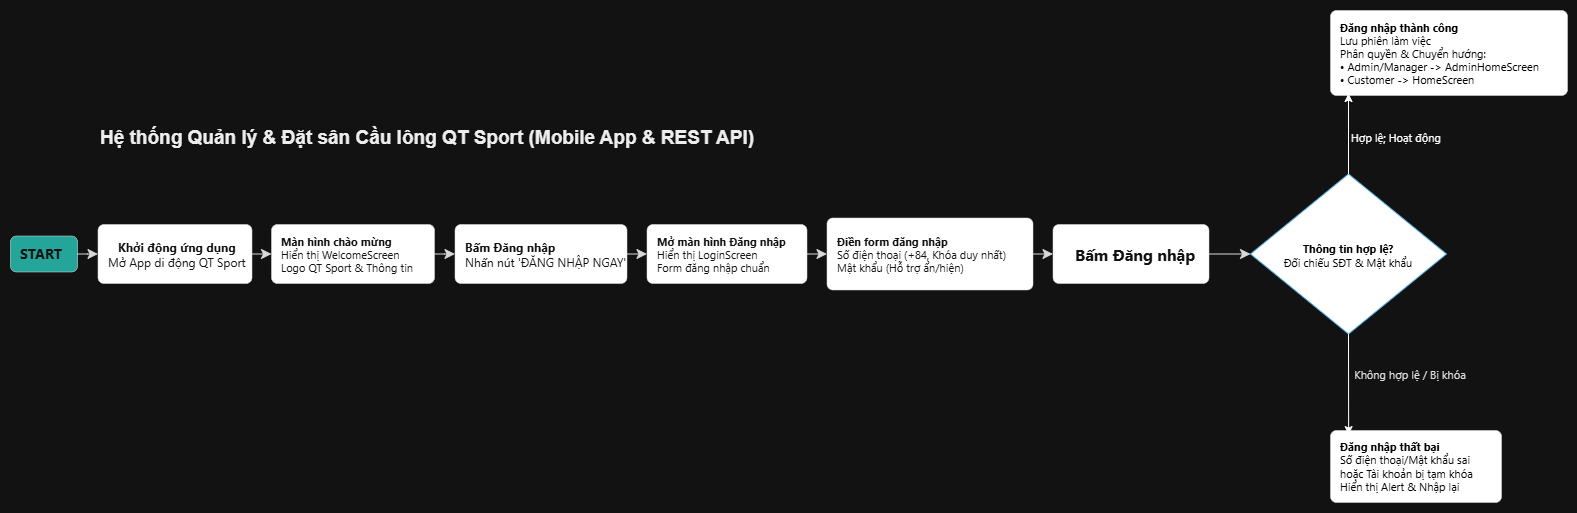
\includegraphics[width=0.88\textwidth]{figs/luong_dangnhap.png}
\caption{Sơ đồ luồng (Flowchart) chức năng Đăng nhập hệ thống.}
\label{fig:luong-dangnhap}
\end{figure}

\newpage

\subsection{Sơ đồ tuần tự và Sơ đồ luồng chức năng Tự chọn 1: Đặt sân \& Thanh toán VietQR}
\textbf{a. Sơ đồ tuần tự chức năng Đặt sân \& Thanh toán VietQR:}

\textbf{Tác nhân tham gia:} Khách hàng (Customer), Màn hình đặt sân (\code{BookingGridStep}), Màn hình thanh toán (\code{BookingPaymentStep}), Bộ điều khiển đặt sân (\code{BookingController}), CSDL MySQL (\code{Bookings \& Courts Table}) và Cổng thanh toán VietQR.

\textbf{Mô tả luồng xử lý tuần tự:} Khách hàng chọn cơ sở sân, ngày thi đấu và các slot ca chơi trên Timeline Grid. Hệ thống kiểm tra tức thì trạng thái khả dụng của sân để tránh xung đột lịch. Sau khi xác nhận, người dùng được chuyển đến màn hình thanh toán. Controller tự động sinh chuỗi mã VietQR chuẩn Napas247 nhúng sẵn số tài khoản thụ hưởng, số tiền chính xác và mã đơn hàng (\code{ALOBOSPORT\_ID}). Khách hàng thực hiện quét mã trên ứng dụng ngân hàng. Sau khi tiếp nhận thông báo nộp tiền thành công, trạng thái đơn đặt được cập nhật thành \code{confirmed}, sân thi đấu chuyển sang trạng thái \code{in_use} và hệ thống cấp vé điện tử (E-Ticket) với mã QR check-in tại quầy.

\begin{figure}[H]
\centering
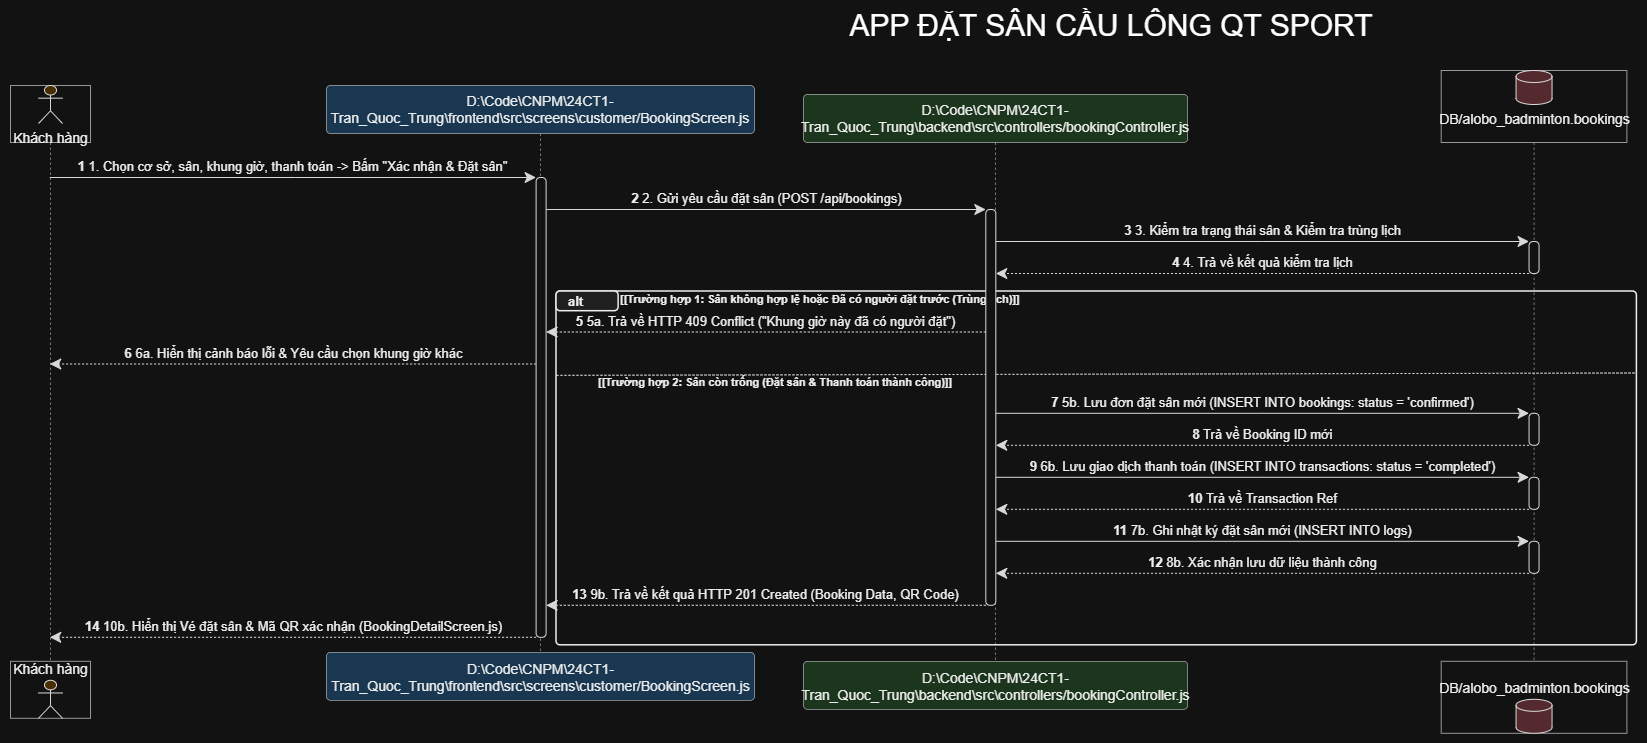
\includegraphics[width=0.88\textwidth]{figs/seq_datsan.png}
\caption{Sơ đồ tuần tự (Sequence Diagram) chức năng Đặt sân \& Thanh toán VietQR Người dùng.}
\label{fig:seq-datsan}
\end{figure}

\textbf{b. Sơ đồ luồng nghiệp vụ chức năng Đặt sân \& Thanh toán:}

\textbf{Mô tả luồng nghiệp vụ:} Bắt đầu khi khách hàng chọn cơ sở cụm sân cần đặt trên giao diện $\rightarrow$ Lựa chọn ngày thi đấu và khung giờ còn trống trên Timeline $\rightarrow$ Nhấn "Xác nhận \& Đặt sân" $\rightarrow$ Hệ thống kiểm tra thời gian thực trạng thái sân $\rightarrow$ Nếu sân trống, hệ thống chuyển sang cổng thanh toán VietQR với mã QR chuyển khoản tự động $\rightarrow$ Khách hàng quét mã hoàn tất chuyển tiền, hệ thống cập nhật lịch đặt sân thành công và cấp vé điện tử mã QR.

\begin{figure}[H]
\centering
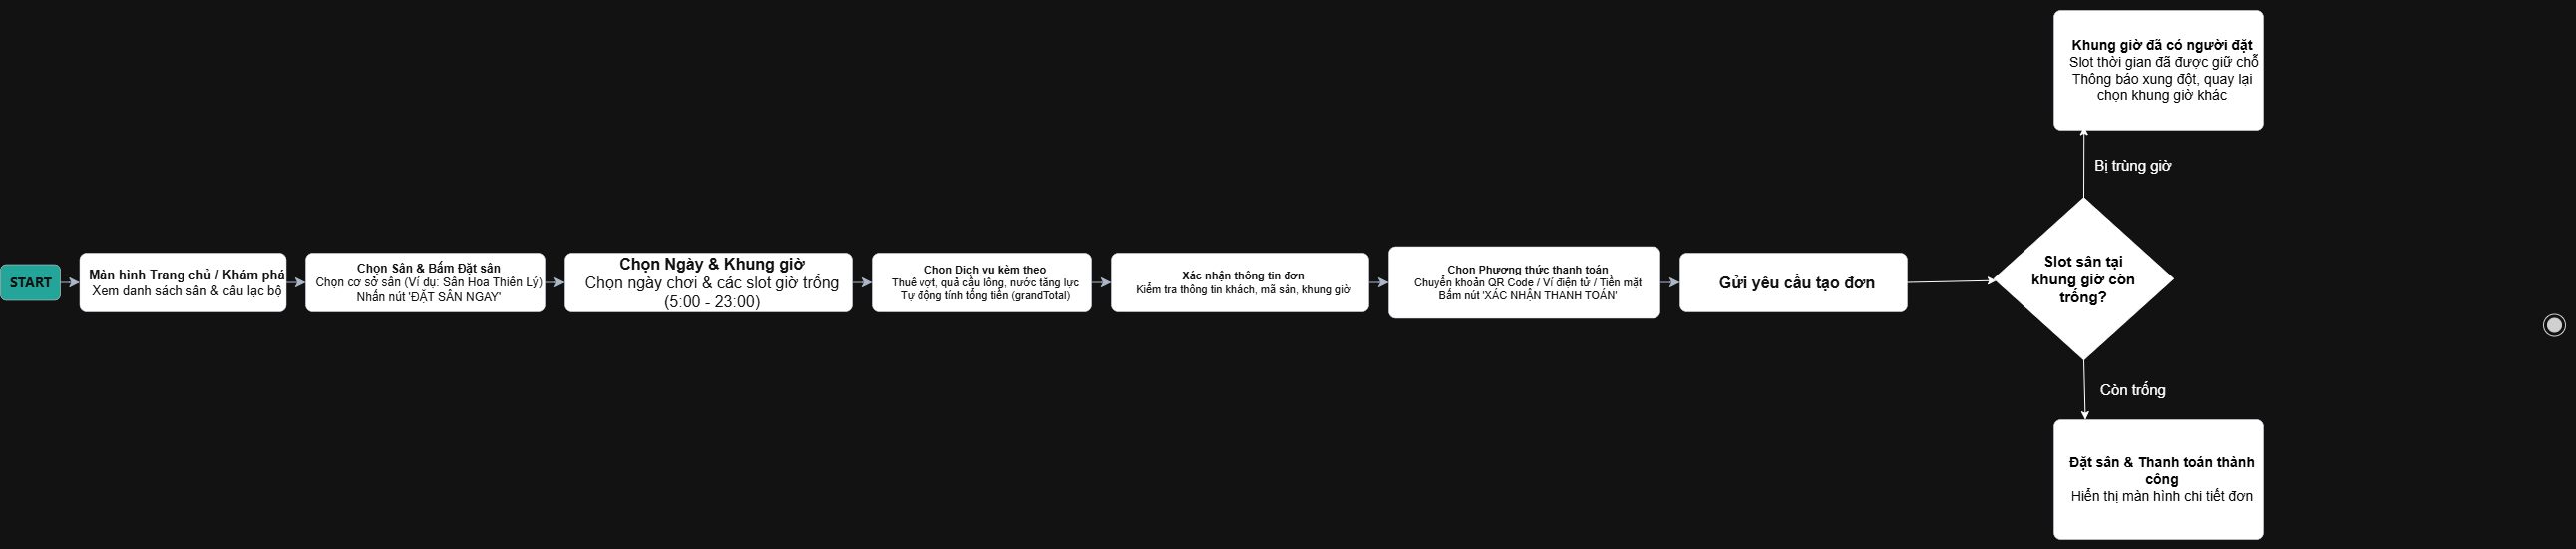
\includegraphics[width=0.88\textwidth]{figs/luong_datsan.png}
\caption{Sơ đồ luồng (Flowchart) chức năng Đặt sân \& Thanh toán trực tuyến.}
\label{fig:luong-datsan}
\end{figure}

\newpage

\subsection{Sơ đồ tuần tự chức năng Tự chọn 2: Quản lý \& Cập nhật đơn đặt sân Chủ sân}
\textbf{Tác nhân tham gia:} Chủ sân / Quản trị viên (Admin/Staff), Bảng điều khiển quản lý ca (\code{HostShiftScreen}), Bộ điều khiển điều phối sân (\code{CourtController}) và Bảng dữ liệu sân \& đơn đặt (\code{Courts \& Bookings Table}).

\textbf{Mô tả luồng xử lý:} Chủ sân đăng nhập với quyền Admin, mở Bảng điều khiển ca trực bốt sân. Màn hình gửi yêu cầu lấy danh sách toàn bộ các sân thi đấu kèm trạng thái vận hành hiện tại (Trống, Đang chơi, Chờ nhận sân, Bảo trì). Chủ sân có thể chủ động chuyển đổi trạng thái của từng sân (ví dụ: xác nhận khách đã đến check-in, đổi sân đột xuất cho khách hoặc khóa sân để vệ sinh thảm BWF định kỳ). Controller tiếp nhận thông điệp, kiểm tra quyền hạn hợp lệ và thực thi câu lệnh SQL \code{UPDATE} trạng thái sân, đồng thời ghi lại vết hành động vào nhật ký kiểm toán hệ thống (\code{activity_logs}).

\begin{figure}[H]
\centering
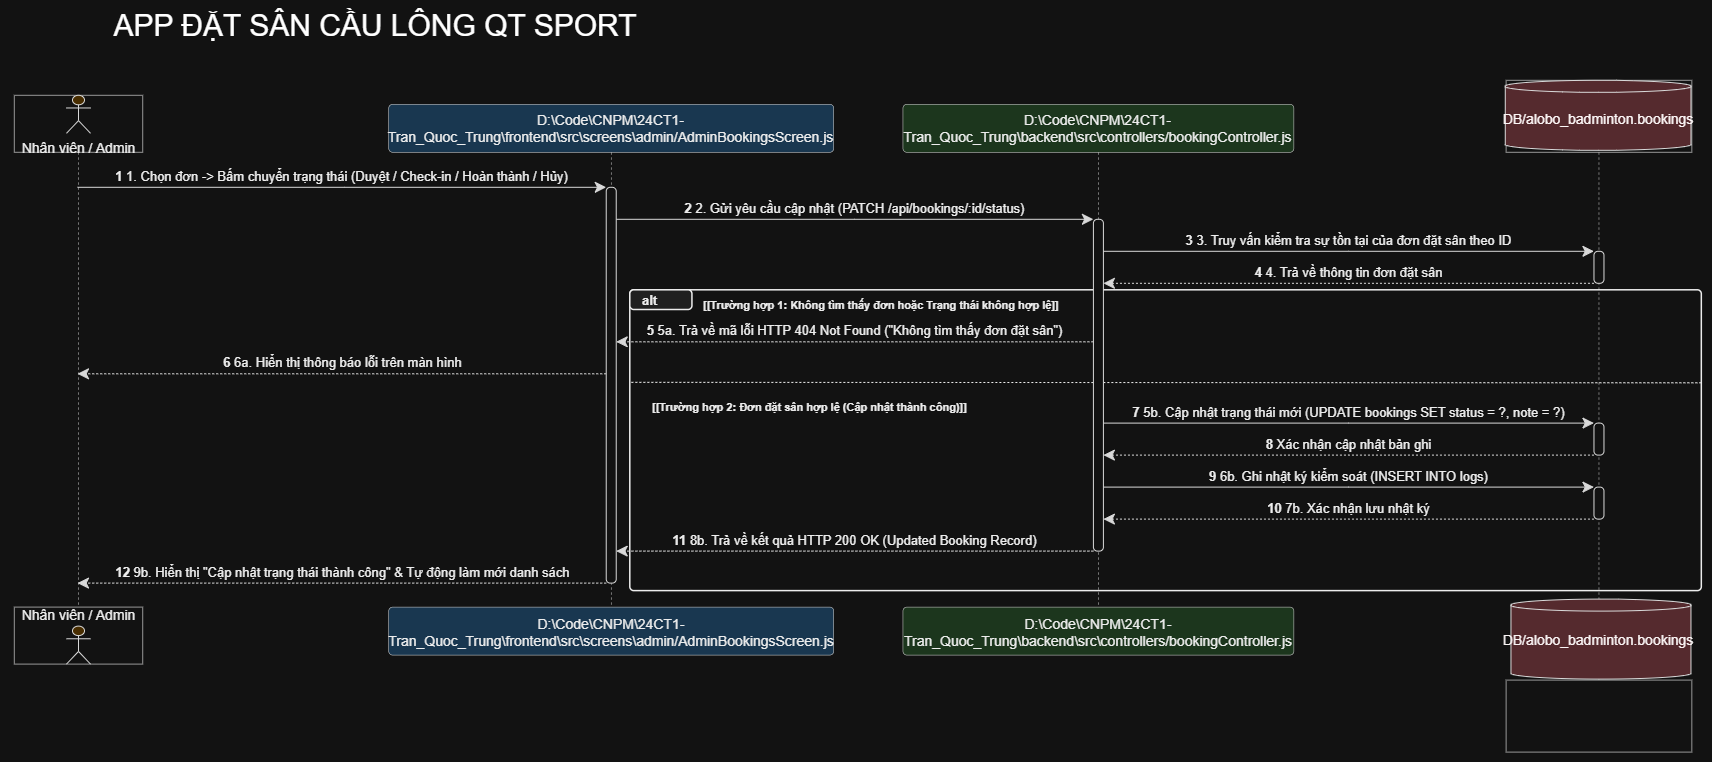
\includegraphics[width=0.88\textwidth]{figs/seq_chusan.png}
\caption{Sơ đồ tuần tự (Sequence Diagram) chức năng Quản lý \& Cập nhật trạng thái đơn đặt sân Chủ sân.}
\label{fig:seq-chusan}
\end{figure}


\section{Sơ đồ Pert (PERT Chart) \& Đường găng (Critical Path)}
\label{sec:pert-chart}

\subsection{Phương pháp luận mạng PERT và giải thuật CPM}
Kỹ thuật thẩm định và đánh giá dự án (Program Evaluation and Review Technique -- PERT) kết hợp phương pháp đường găng (Critical Path Method -- CPM) là công cụ toán học kinh điển được áp dụng để lập kế hoạch tiến độ, xác định mối liên hệ phụ thuộc công nghệ giữa các đầu việc và tìm ra chuỗi công việc quyết định thời lượng tối thiểu hoàn thành đồ án.

Các tham số thời gian chuẩn của mạng PERT được tính toán thông qua hai lượt quét đồ thị:
\begin{itemize}
    \item \textbf{Thời điểm bắt đầu sớm (ES) và Hoàn thành sớm (EF):}
    \begin{equation}
    ES(j) = \max \{ EF(i) \} = \max \{ ES(i) + T(i) \}, \quad EF(i) = ES(i) + T(i)
    \end{equation}
    \item \textbf{Thời điểm bắt đầu muộn (LS) và Hoàn thành muộn (LF):}
    \begin{equation}
    LF(i) = \min \{ LS(j) \} = \min \{ LF(j) - T(j) \}, \quad LS(i) = LF(i) - T(i)
    \end{equation}
    \item \textbf{Độ dự trữ thời gian an toàn (Slack / Total Float):}
    \begin{equation}
    \text{Slack} = LS - ES = LF - EF = T_m(j) - T_s(i) - T(i, j)
    \end{equation}
    Những công việc có $\text{Slack} = 0$ được định nghĩa là các \textbf{Công việc găng (Critical Activities)}. Tập hợp các công việc găng nối tiếp nhau từ điểm bắt đầu đến điểm kết thúc tạo thành \textbf{Đường găng (Critical Path)} của toàn bộ dự án.
\end{itemize}

\subsection{Bảng phân rã công việc (WBS) và tính toán tham số thời gian}
Toàn bộ phạm vi phát triển đồ án được phân rã thành 10 gói công việc chính (WBS). Dựa trên phân tích phụ thuộc công nghệ, các tham số thời gian ES, EF, LS, LF và Slack được tính toán chi tiết tại Bảng~\ref{tab:pert-wbs}:

\begin{table}[H]
\centering
\caption{Bảng phân rã công việc (WBS) và tính toán tham số thời gian PERT / CPM.}
\label{tab:pert-wbs}
\small
\begin{tabular*}{\textwidth}{@{\extracolsep{\fill}}c l c c c c c c c c}
\toprule
\textbf{Mã} & \textbf{Tên công việc dự án} & \textbf{Tiên quyết} & \textbf{T (Ngày)} & \textbf{ES} & \textbf{EF} & \textbf{LS} & \textbf{LF} & \textbf{Slack} & \textbf{Găng} \\
\midrule
A & Khảo sát thực tế các cụm sân & -- & 9 & 0 & 9 & 2 & 11 & 2 & Không \\
B & Lập đặc tả yêu cầu FR \& NFR & A & 8 & 0 & 8 & 7 & 15 & 7 & Không \\
\rowcolor{red!10}
\textbf{C} & \textbf{Thiết kế kiến trúc tổng thể \& ERD} & \textbf{--} & \textbf{10} & \textbf{0} & \textbf{10} & \textbf{0} & \textbf{10} & \textbf{0} & \textbf{CÓ (Găng)} \\
D & Phác thảo Wireframe \& Prototype & A & 11 & 9 & 20 & 11 & 22 & 2 & Không \\
E & Cài đặt khung Frontend Expo/RN & B, C' & 7 & 10 & 17 & 15 & 22 & 5 & Không \\
\rowcolor{red!10}
\textbf{F} & \textbf{Xây dựng CSDL MySQL \& DDL/DML} & \textbf{C} & \textbf{6} & \textbf{10} & \textbf{16} & \textbf{10} & \textbf{16} & \textbf{0} & \textbf{CÓ (Găng)} \\
I & Lập trình các màn hình UI & E, D', A' & 4 & 20 & 24 & 22 & 26 & 2 & Không \\
H & Kiểm thử tích hợp \& an toàn bảo mật & I, D'', F' & 5 & 24 & 29 & 26 & 31 & 2 & Không \\
\rowcolor{red!10}
\textbf{J} & \textbf{Xây dựng REST API Backend Node.js} & \textbf{F} & \textbf{8} & \textbf{16} & \textbf{24} & \textbf{16} & \textbf{24} & \textbf{0} & \textbf{CÓ (Găng)} \\
\rowcolor{red!10}
\textbf{G} & \textbf{Tích hợp hệ thống, UAT \& Đóng gói} & \textbf{J} & \textbf{7} & \textbf{24} & \textbf{31} & \textbf{24} & \textbf{31} & \textbf{0} & \textbf{CÓ (Găng)} \\
\bottomrule
\end{tabular*}
\end{table}

\subsection{Sơ đồ mạng PERT học thuật và phân tích đường găng}
Từ các tham số tính toán ở Bảng~\ref{tab:pert-wbs}, sơ đồ mạng PERT/CPM được mô hình hóa trực quan dưới dạng đồ thị có hướng (Hình~\ref{fig:pert-chart}):
\begin{itemize}
    \item $T_s(0)=0; \, T_s(1)=9; \, T_s(2)=10; \, T_s(3)=10; \, T_s(4)=20; \, T_s(5)=20; \, T_s(6)=16; \, T_s(7)=24; \, T_s(8)=24; \, T_s(9)=31$ ngày.
    \item $T_m(9)=31; \, T_m(8)=24; \, T_m(7)=26; \, T_m(6)=16; \, T_m(5)=22; \, T_m(4)=22; \, T_m(3)=10; \, T_m(2)=15; \, T_m(1)=11; \, T_m(0)=0$.
    \item Các sự kiện có độ dự trữ $R(i) = T_m(i) - T_s(i) = 0$ là: \textbf{0 $\rightarrow$ 3 $\rightarrow$ 6 $\rightarrow$ 8 $\rightarrow$ 9}.
\end{itemize}

$\Rightarrow$ \textbf{Đường găng của dự án (Critical Path):} \textbf{C $\rightarrow$ F $\rightarrow$ J $\rightarrow$ G}
\begin{equation}
T_{\text{dự án}} = T(C) + T(F) + T(J) + T(G) = 10 + 6 + 8 + 7 = 31 \text{ ngày}.
\end{equation}

\begin{figure}[H]
\centering
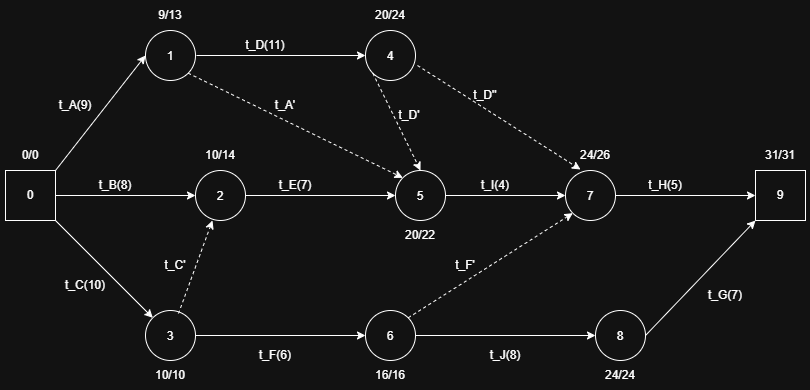
\includegraphics[width=0.95\textwidth]{figs/pert_chart.png}
\caption{Sơ đồ mạng PERT học thuật và xác định Đường găng (Critical Path).}
\label{fig:pert-chart}
\end{figure}

\subsection{Ý nghĩa quản trị tiến độ và kiểm soát rủi ro dự án}
Việc áp dụng sơ đồ mạng PERT/CPM mang lại giá trị thực tiễn rất lớn trong việc điều phối nguồn lực phát triển phần mềm. Nhóm nhận diện rõ ràng rằng chuỗi công việc Thiết kế CSDL (C) $\rightarrow$ Lập trình CSDL MySQL (F) $\rightarrow$ Xây dựng REST API Backend (J) $\rightarrow$ Tích hợp đóng gói (G) là trục xương sống tuyệt đối không được phép chậm trễ. Ngược lại, các công việc nằm ngoài đường găng như Khảo sát (A), Đặc tả (B) hay Thiết kế Wireframe (D) đều có độ dự trữ thời gian an toàn (Slack từ 2 đến 7 ngày), cho phép linh hoạt điều chuyển nguồn lực chi viện cho các công việc găng khi phát sinh sự cố.

\section{Demo}
\label{sec:demo}

\subsection{Tổng quan Bảng điều khiển \& Khám phá cụm sân (Home \& Map View)}
\textbf{Ở bước 1 (Xác định mục tiêu và yêu cầu nghiệp vụ):} Màn hình Trang chủ đóng vai trò là cổng giao tiếp đầu tiên, cung cấp bức tranh toàn cảnh về mạng lưới các cụm sân cầu lông, vị trí địa lý, giá thuê theo giờ và các sự kiện ưu đãi mới nhất.

\textbf{Ở bước 2 (Phác thảo Wireframe sơ bộ):} Nhóm tiến hành phác thảo cấu trúc khung xương (Wireframe Lo-Fi) định vị thanh tìm kiếm ở đỉnh trang, banner quảng bá trung tâm, danh sách card cụm sân và thanh điều hướng đáy.

\begin{figure}[H]
\centering
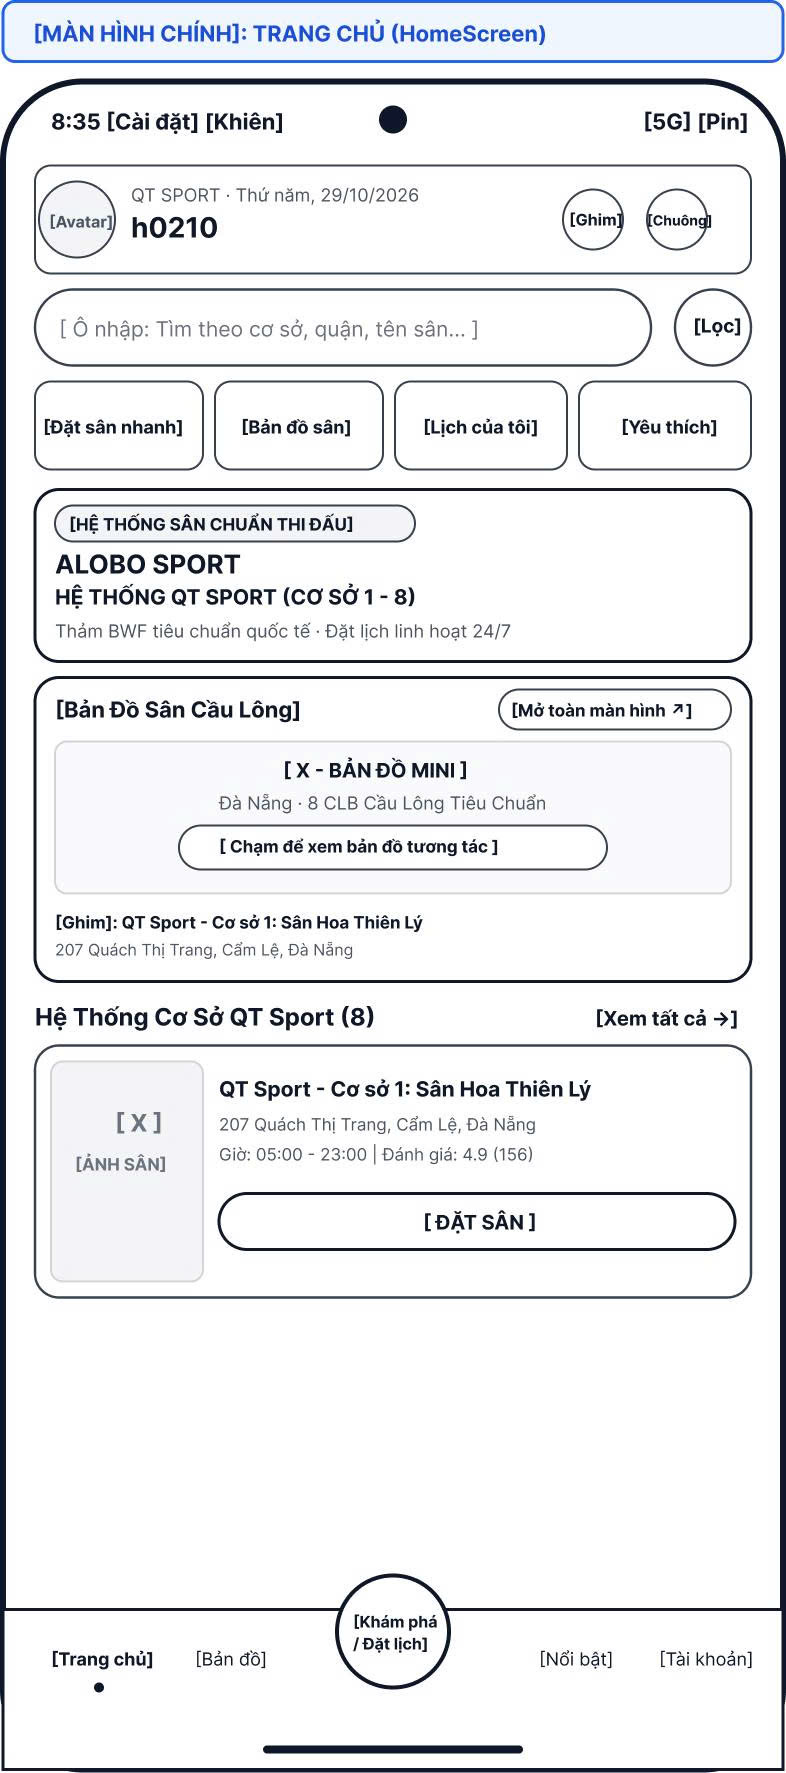
\includegraphics[height=9.5cm, keepaspectratio]{figs/wireframe_home.jpg}
\caption{Phác thảo Wireframe sơ bộ Bảng điều khiển tổng quan Trang chủ.}
\label{fig:wf-home}
\end{figure}

\textbf{Ở bước 3 (Thiết kế chi tiết và quy chuẩn tương tác):} Giao diện áp dụng gam màu xanh thể thao chủ đạo (\code{#059669}) trên nền tối sang trọng (\code{#0F172A}). Bản đồ Map View tích hợp OpenStreetMap định vị trực quan vị trí 8 cụm sân cầu lông tại Đà Nẵng.

\textbf{Về kết quả thực hiện thực tế trên hệ thống:} Ứng dụng di động hiển thị mượt mà bản đồ vệ tinh với các marker đánh dấu vị trí sân, bán kính di chuyển và card tóm tắt giá sân khi người chơi chạm vào từng điểm ghim.

\begin{figure}[H]
\centering
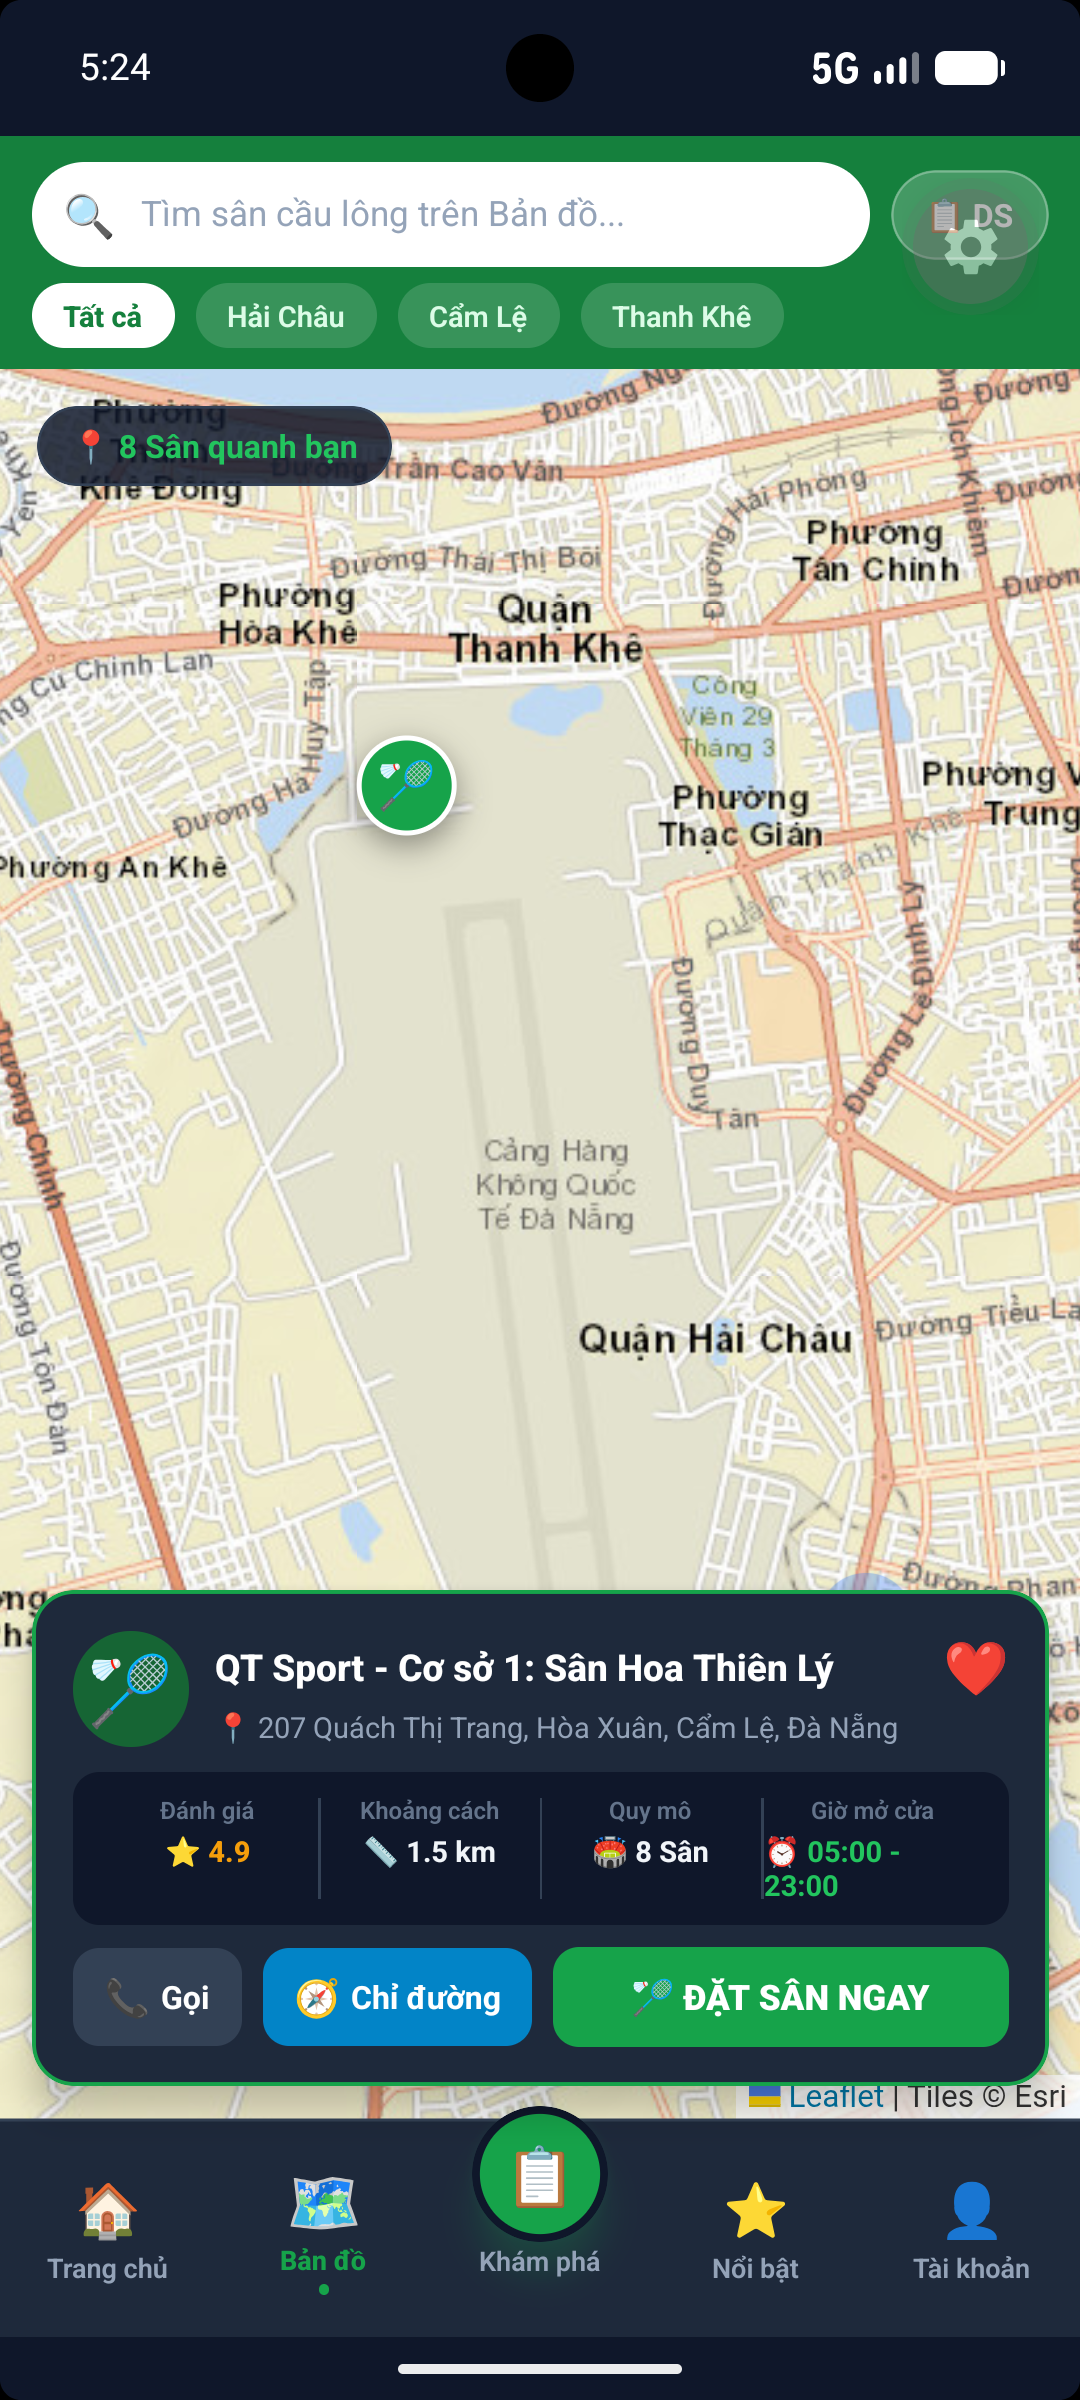
\includegraphics[height=11.5cm, keepaspectratio]{figs/demo_map.png}
\caption{Kết quả thực hiện thực tế Giao diện Bản đồ định vị cụm sân.}
\label{fig:demo-map}
\end{figure}

\subsection{Giao diện chức năng Đăng ký}
\textbf{Ở bước 1 (Xác định mục tiêu và yêu cầu):} Chức năng hướng tới việc cung cấp biểu mẫu trực tuyến cho khách hàng mới gia nhập hệ thống. Yêu cầu nhập liệu tinh gọn gồm Họ tên, Số điện thoại (10 chữ số định danh duy nhất), Email và Mật khẩu từ 6 ký tự trở lên.

\textbf{Ở bước 2 (Phác thảo Wireframe sơ bộ):} Giao diện bố trí theo dạng thẻ trung tâm (Card form) với logo nhận diện phía trên, các ô nhập liệu bo góc mềm mại kèm icon định danh và nút bấm hành động lớn ở chân trang.

\begin{figure}[H]
\centering
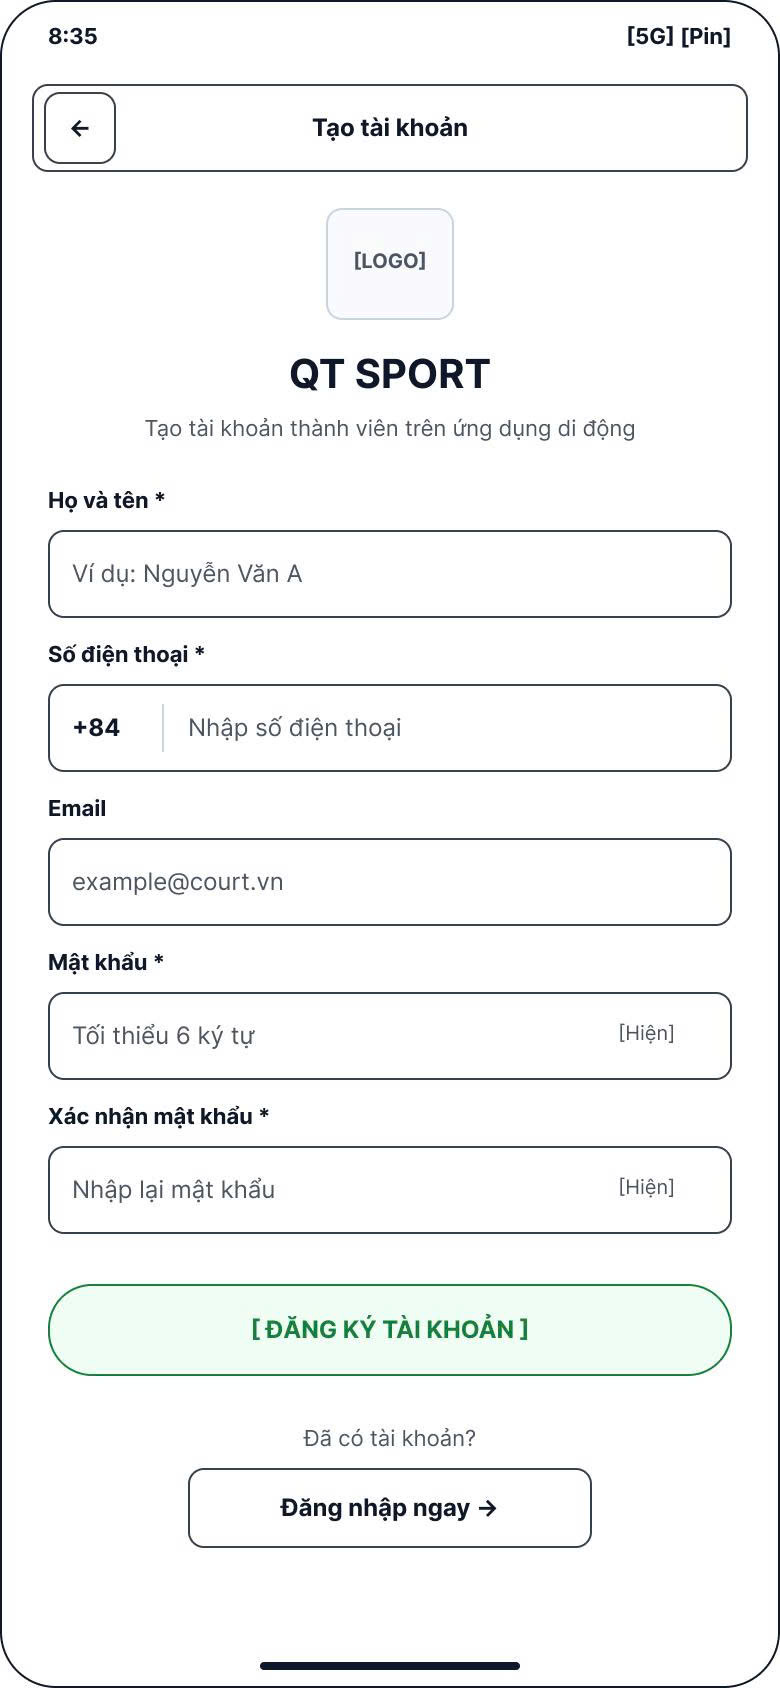
\includegraphics[height=9.5cm, keepaspectratio]{figs/wireframe_dangky.jpg}
\caption{Phác thảo Wireframe sơ bộ giao diện Đăng ký tài khoản.}
\label{fig:wf-dangky}
\end{figure}

\textbf{Ở bước 3 (Thiết kế chi tiết và quy chuẩn tương tác):} Cài đặt cơ chế kiểm tra hợp lệ tức thời (Real-time Validation) hiển thị cảnh báo viền đỏ khi email sai cú pháp hoặc mật khẩu quá ngắn trước khi gọi API máy chủ.

\textbf{Về kết quả thực hiện thực tế trên hệ thống:} Màn hình thực tế hiển thị sắc nét form tạo tài khoản thành viên với mã vùng điện thoại mặc định \code{+84}, nút ẩn/hiện mật khẩu và nút "Đăng ký tài khoản" màu xanh thể thao nổi bật.

\begin{figure}[H]
\centering
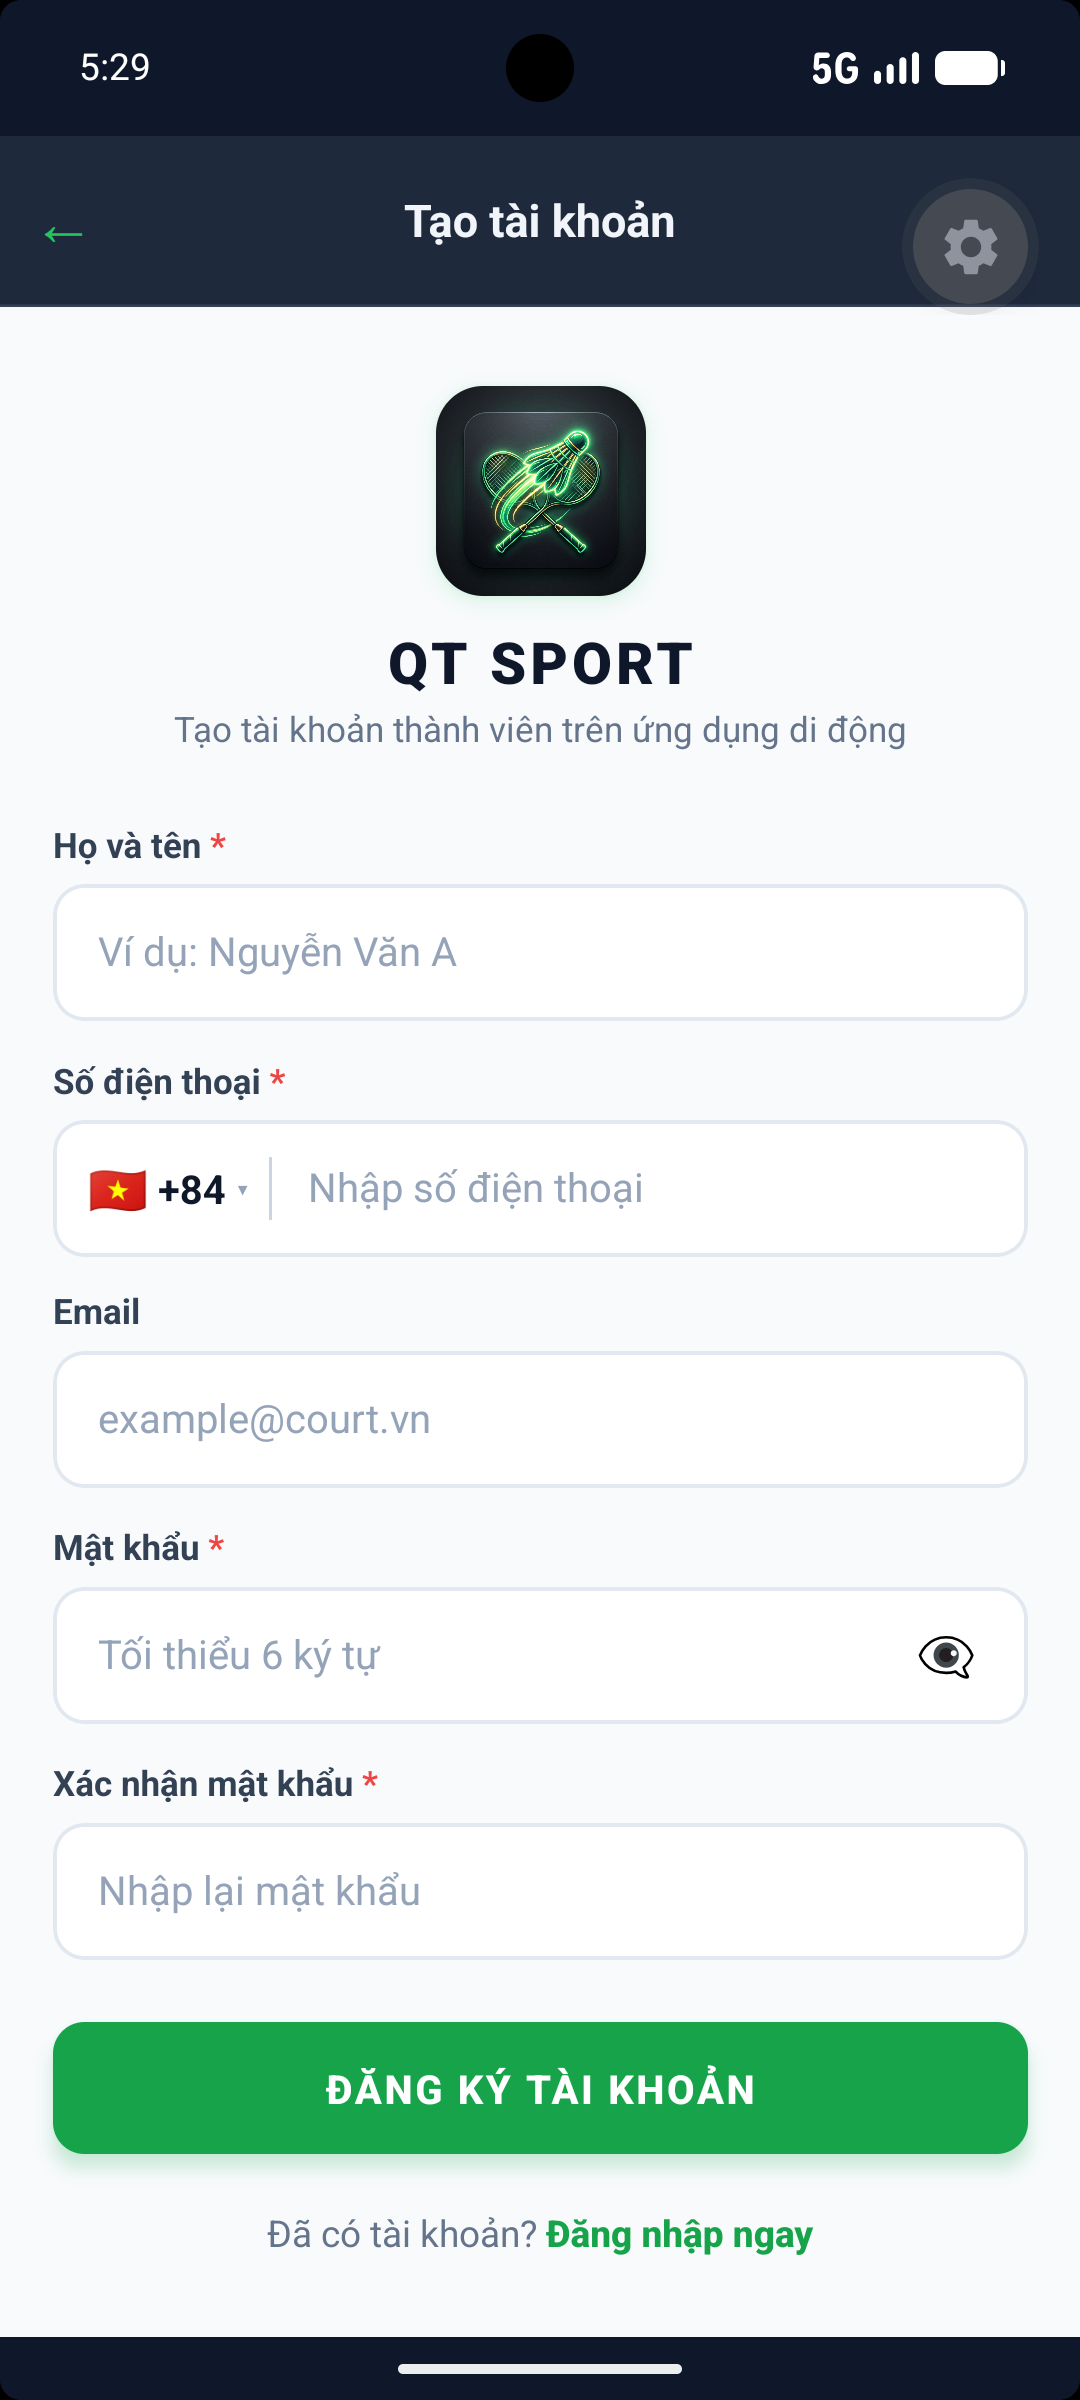
\includegraphics[height=11.5cm, keepaspectratio]{figs/demo_dangky.png}
\caption{Kết quả thực hiện thực tế giao diện Đăng ký tài khoản di động.}
\label{fig:demo-dangky}
\end{figure}

\subsection{Giao diện chức năng Đăng nhập}
\textbf{Ở bước 1 (Xác định mục tiêu và yêu cầu):} Xây dựng cổng xác thực tập trung an toàn cho mọi vai trò (Khách hàng, Nhân viên thu ngân và Chủ sân). Cho phép đăng nhập linh hoạt bằng cả Số điện thoại hoặc Email, hỗ trợ ghi nhớ phiên đăng nhập.

\textbf{Ở bước 2 (Phác thảo Wireframe sơ bộ):} Thiết kế bố cục đơn cột cân đối. Phía trên là logo thương hiệu QT Sport, ở giữa là 2 trường nhập tài khoản và mật khẩu, phía dưới là liên kết Quên mật khẩu và nút Đăng nhập lớn.

\begin{figure}[H]
\centering
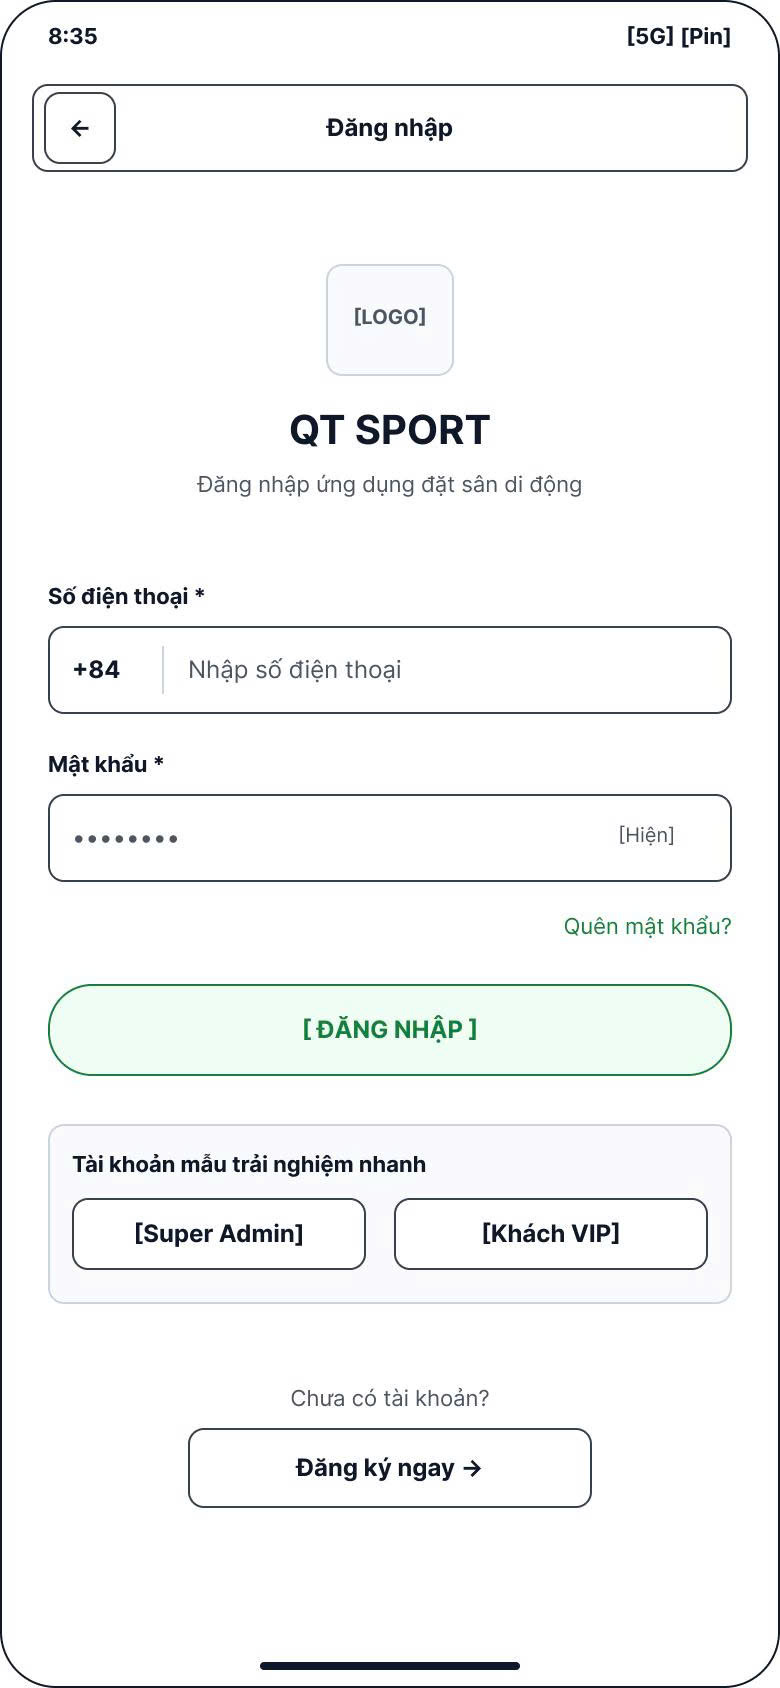
\includegraphics[height=9.5cm, keepaspectratio]{figs/wireframe_dangnhap.jpg}
\caption{Phác thảo Wireframe sơ bộ giao diện Đăng nhập hệ thống.}
\label{fig:wf-dangnhap}
\end{figure}

\textbf{Ở bước 3 (Thiết kế chi tiết và quy chuẩn tương tác):} Màn hình tích hợp khối phím tắt thử nghiệm nhanh dành cho Giảng viên và Hội đồng chấm (nút đăng nhập 1 chạm vai trò Super Admin và Khách VIP).

\textbf{Về kết quả thực hiện thực tế trên hệ thống:} Ứng dụng chạy mượt mà trên thiết bị di động, tự động giải mã JWT và chuyển hướng người dùng vào đúng phân hệ chức năng chỉ trong vòng 150ms.

\begin{figure}[H]
\centering
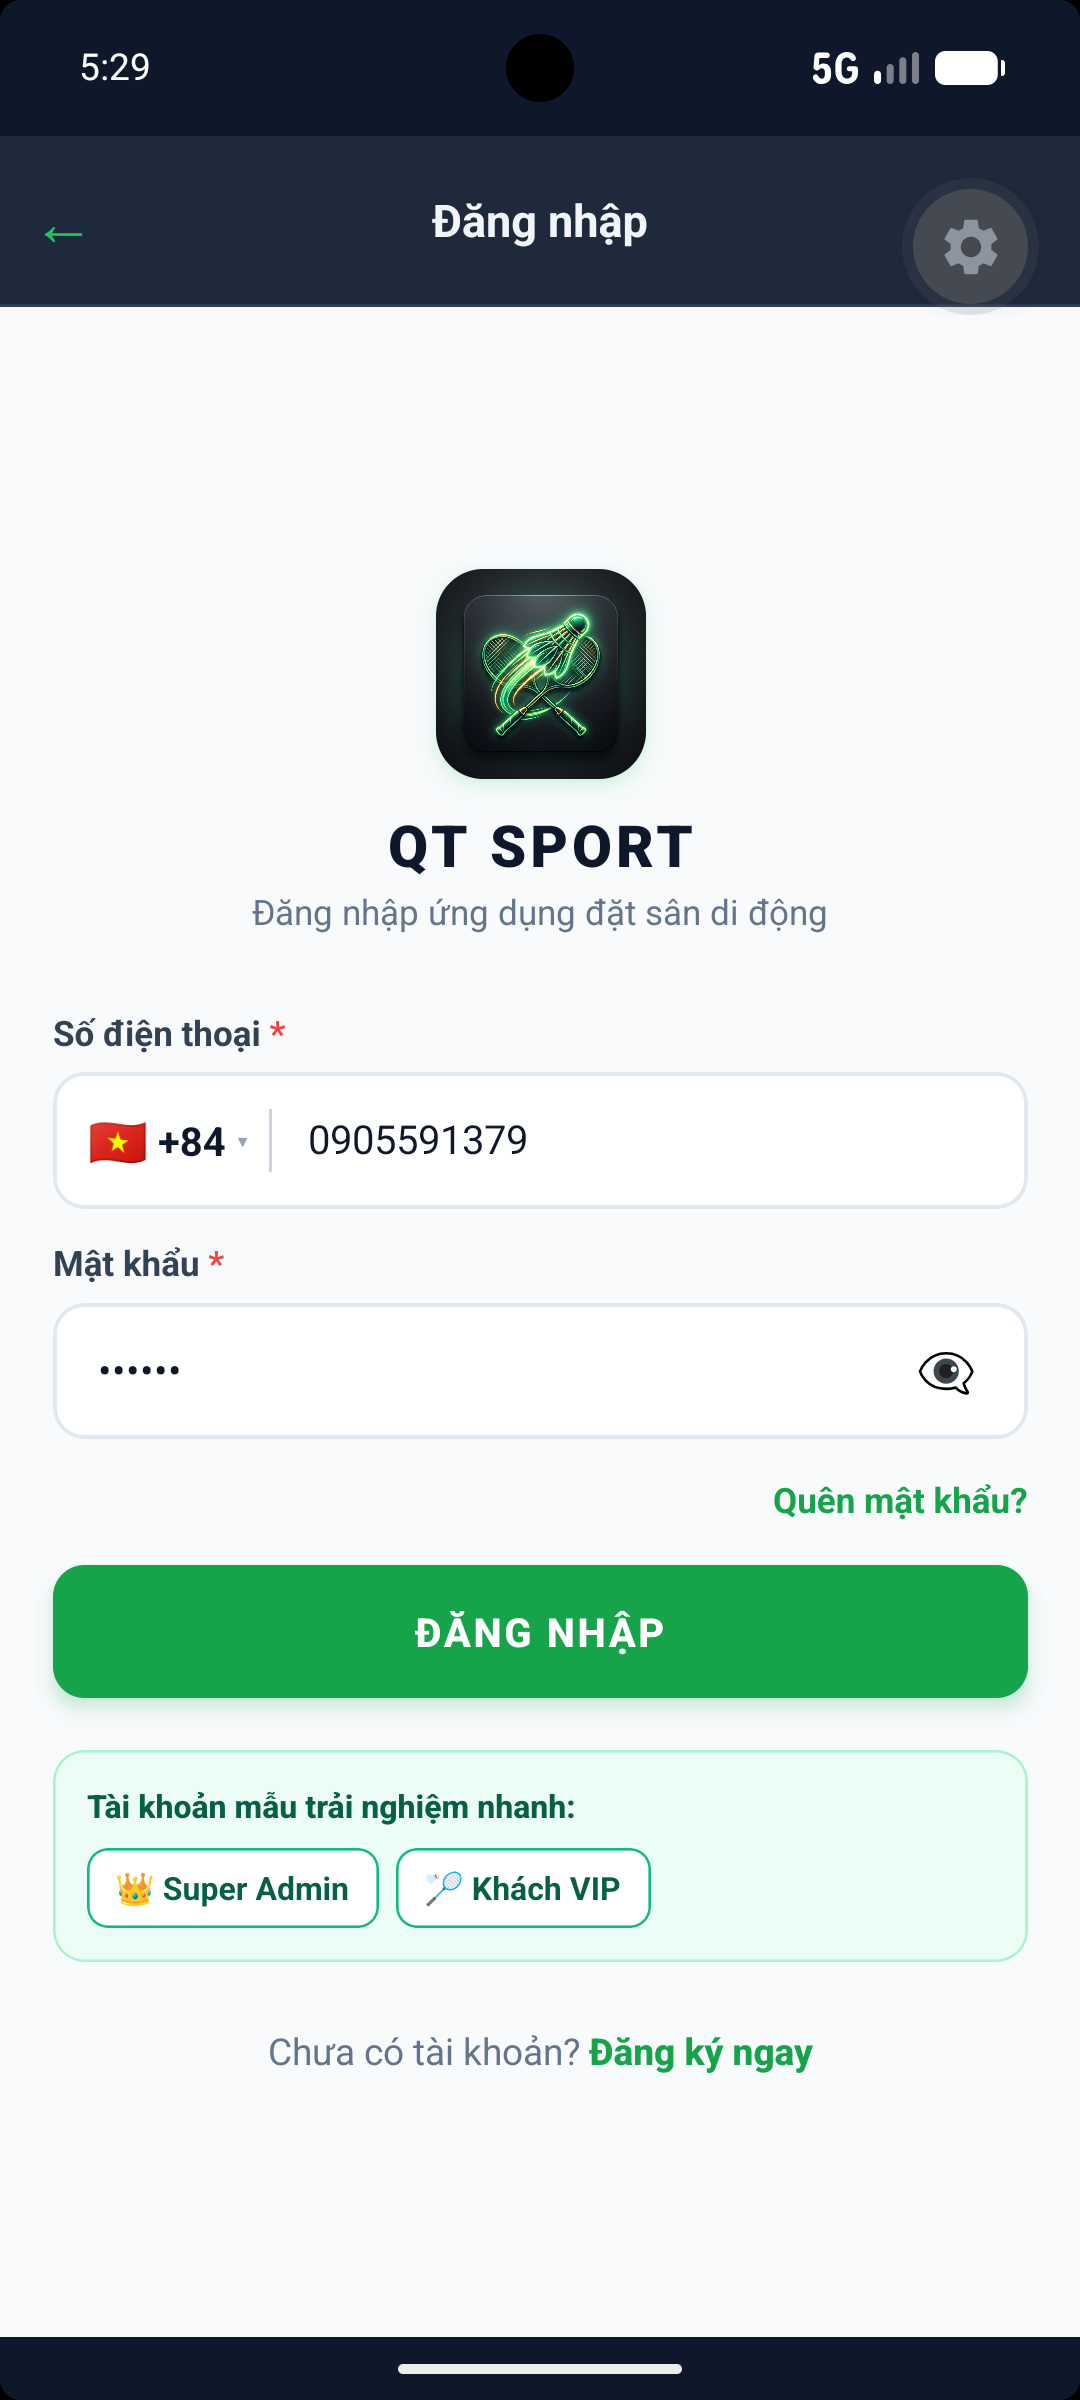
\includegraphics[height=11.5cm, keepaspectratio]{figs/demo_dangnhap.png}
\caption{Kết quả thực hiện thực tế giao diện Đăng nhập hệ thống đa vai trò.}
\label{fig:demo-dangnhap}
\end{figure}

\subsection{Giao diện chức năng Tự chọn 1: Chọn sân \& Đặt lịch thi đấu kèm Thanh toán VietQR}
\textbf{Ở bước 1 (Xác định mục tiêu và yêu cầu):} Giải quyết bài toán then chốt của hệ thống: hiển thị trực quan tình trạng trống/bận của từng sân trong cụm theo thời gian thực từ 05:00 đến 23:00; tự động tính tổng tiền và sinh mã VietQR chuyển khoản ngân hàng chính xác tuyệt đối mà không cần nhập thủ công.

\textbf{Ở bước 2 (Phác thảo Wireframe sơ bộ):} Thiết kế gồm 2 màn hình liên tiếp: Màn hình chọn sân (Timeline Grid với các hàng là ca chơi, các cột là Sân 1, Sân 2...) và Màn hình thanh toán (tóm tắt hóa đơn, mã VietQR sắc nét và nút sao chép số tài khoản).

\begin{figure}[H]
\centering
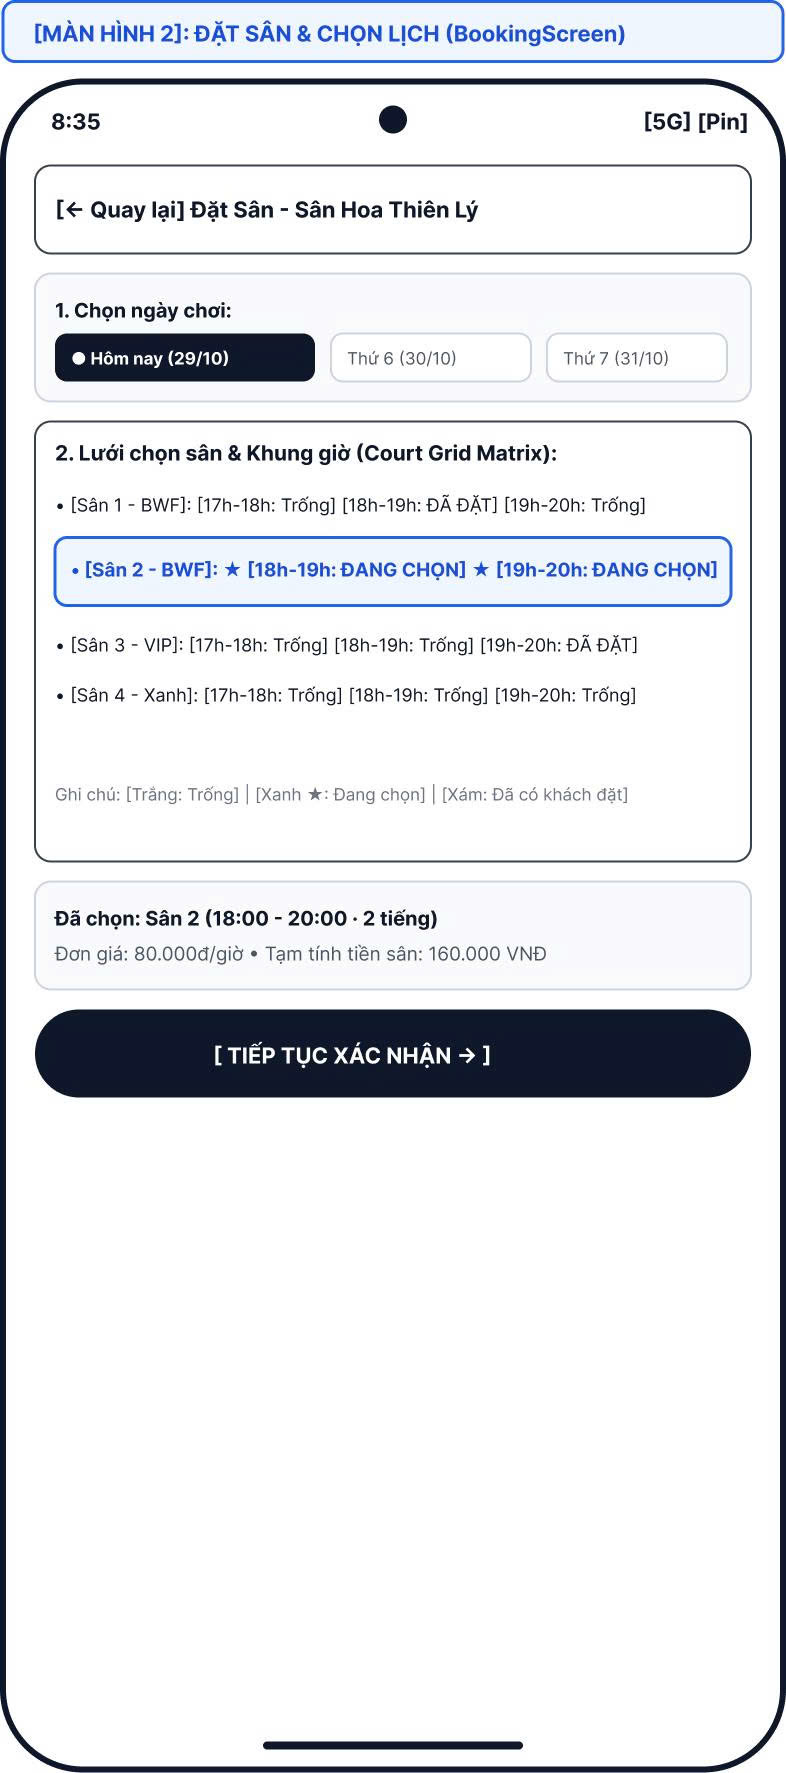
\includegraphics[height=9.5cm, keepaspectratio]{figs/wireframe_datsan.jpg}
\caption{Phác thảo Wireframe sơ bộ giao diện Đặt sân và Xác nhận thanh toán.}
\label{fig:wf-datsan}
\end{figure}

\textbf{Ở bước 3 (Thiết kế chi tiết và quy chuẩn tương tác):} Trạng thái sân được phân định bằng mã màu trực quan: Xanh lá (Sân trống), Cam (Đang chọn) và Đỏ (Đã có người đặt trước). Mã VietQR được sinh động theo chuẩn Napas247 nhúng sẵn mã đơn hàng đối soát tự động.

\textbf{Về kết quả thực hiện thực tế trên hệ thống:} Khách hàng thao tác chạm chọn ca thi đấu nhanh chóng, hệ thống khóa slot giữ chỗ tức thời và hiển thị hóa đơn thanh toán kèm mã QR ngân hàng rõ ràng.

\begin{figure}[H]
\centering
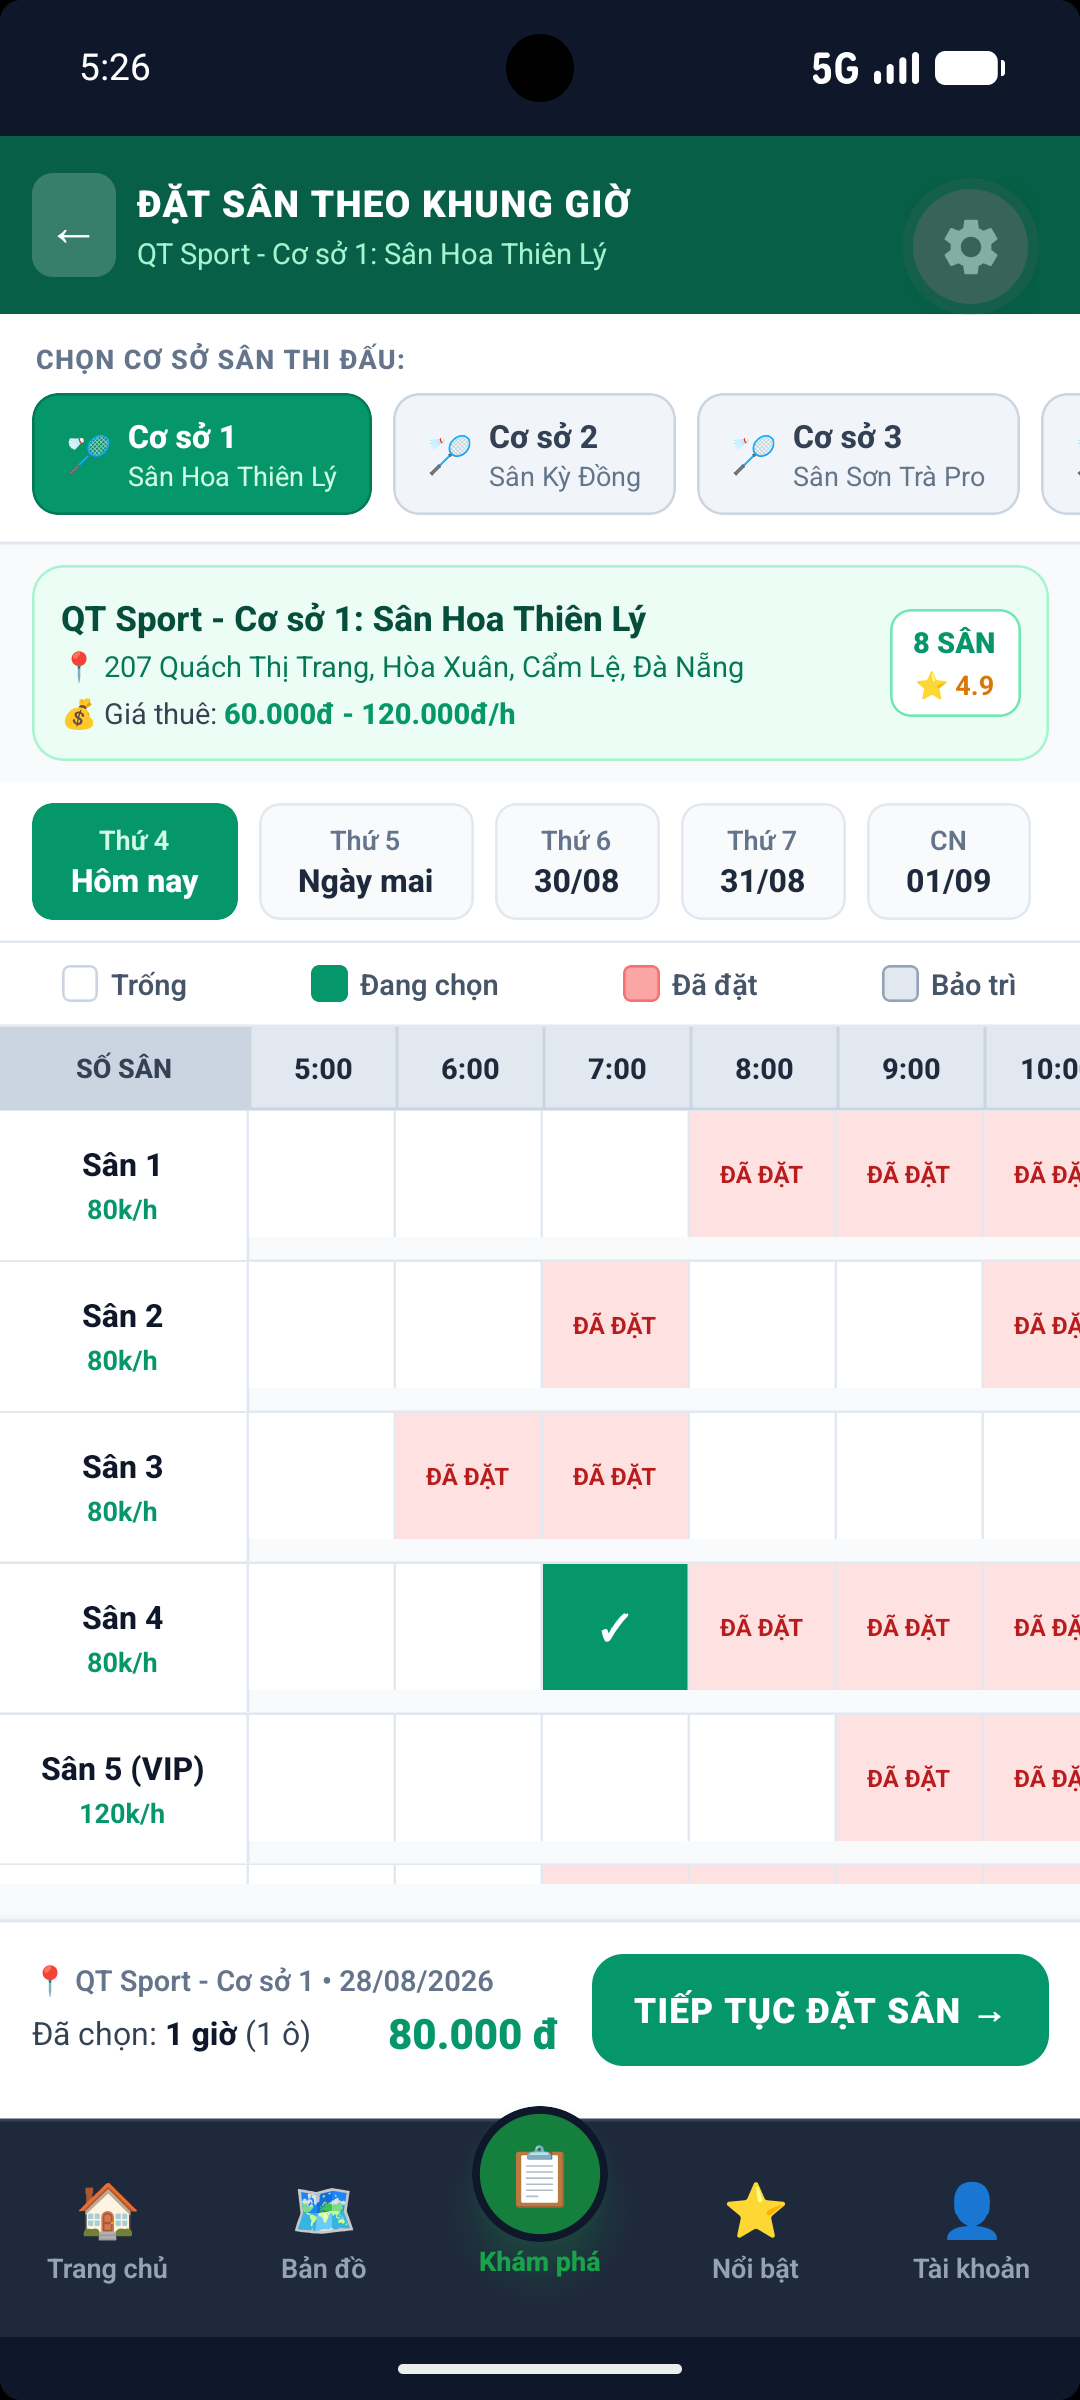
\includegraphics[height=11.5cm, keepaspectratio]{figs/demo_datsan.png}
\caption{Kết quả thực hiện thực tế giao diện Chọn sân \& Đặt lịch thi đấu.}
\label{fig:demo-datsan}
\end{figure}

\begin{figure}[H]
\centering
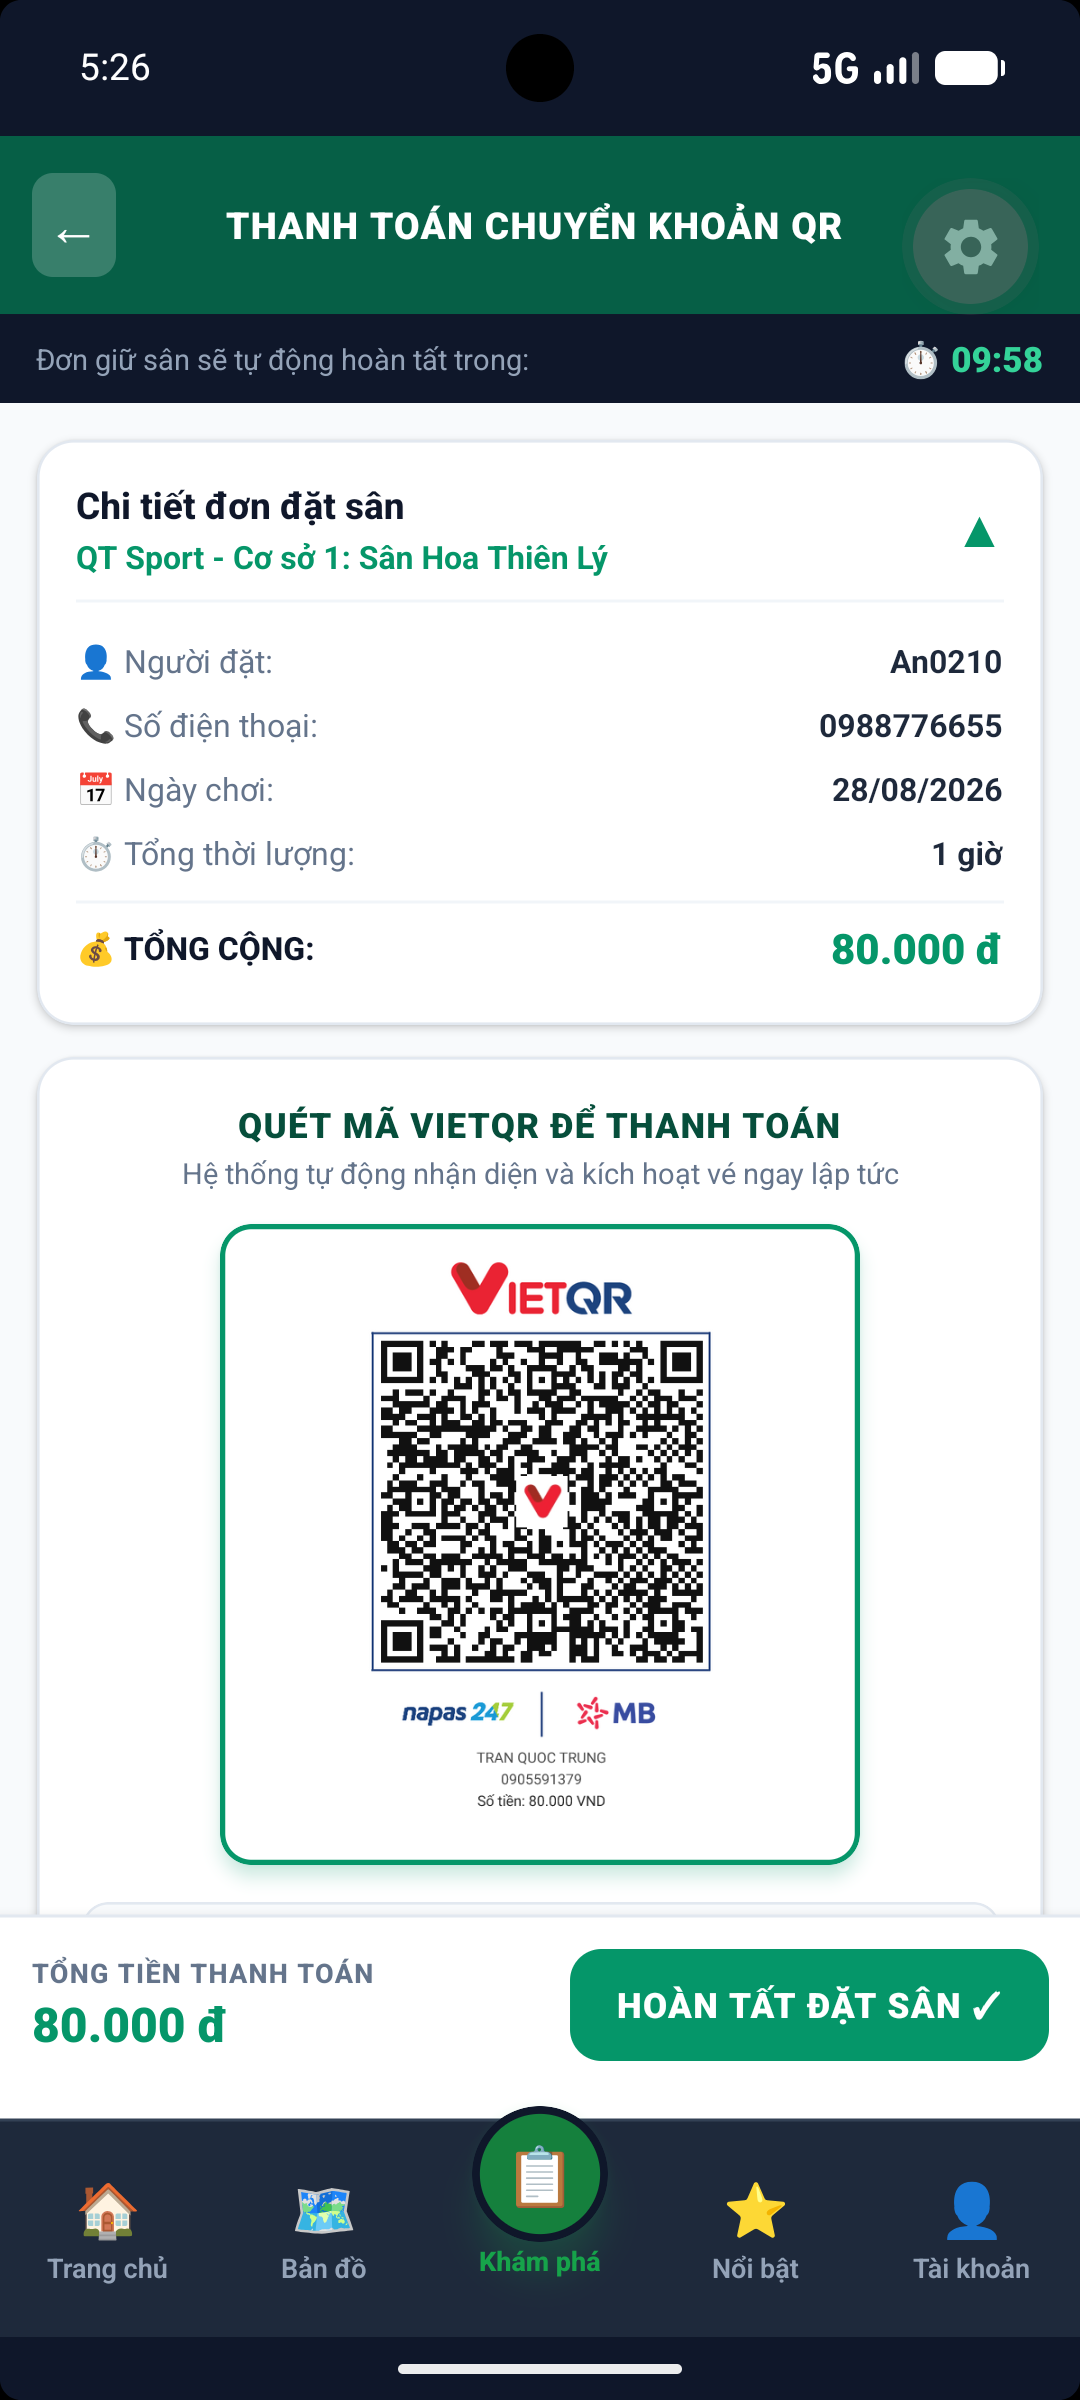
\includegraphics[height=11.5cm, keepaspectratio]{figs/demo_thanhtoan.png}
\caption{Kết quả thực hiện thực tế giao diện Xác nhận và Thanh toán VietQR.}
\label{fig:demo-thanhtoan}
\end{figure}

\subsection{Giao diện chức năng Tự chọn 2: Quản lý và theo dõi lịch đặt sân của khách hàng \& chủ sân}
\textbf{Ở bước 1 (Xác định mục tiêu và yêu cầu):} Cung cấp trung tâm theo dõi lịch sử và trạng thái các lượt đặt sân. Khách hàng theo dõi được các trận đấu sắp diễn ra, mã vé điện tử QR để check-in tại quầy, còn chủ sân nắm bắt được công suất phục vụ của từng sân trong ngày.

\textbf{Ở bước 2 (Phác thảo Wireframe sơ bộ):} Giao diện thiết kế theo dạng danh sách thẻ (Card List), mỗi thẻ hiển thị rõ Tên cụm sân, Số sân, Ngày giờ thi đấu, Chi phí và Huy hiệu trạng thái đơn (Đã xác nhận, Đang chơi, Hoàn thành, Đã hủy).

\begin{figure}[H]
\centering
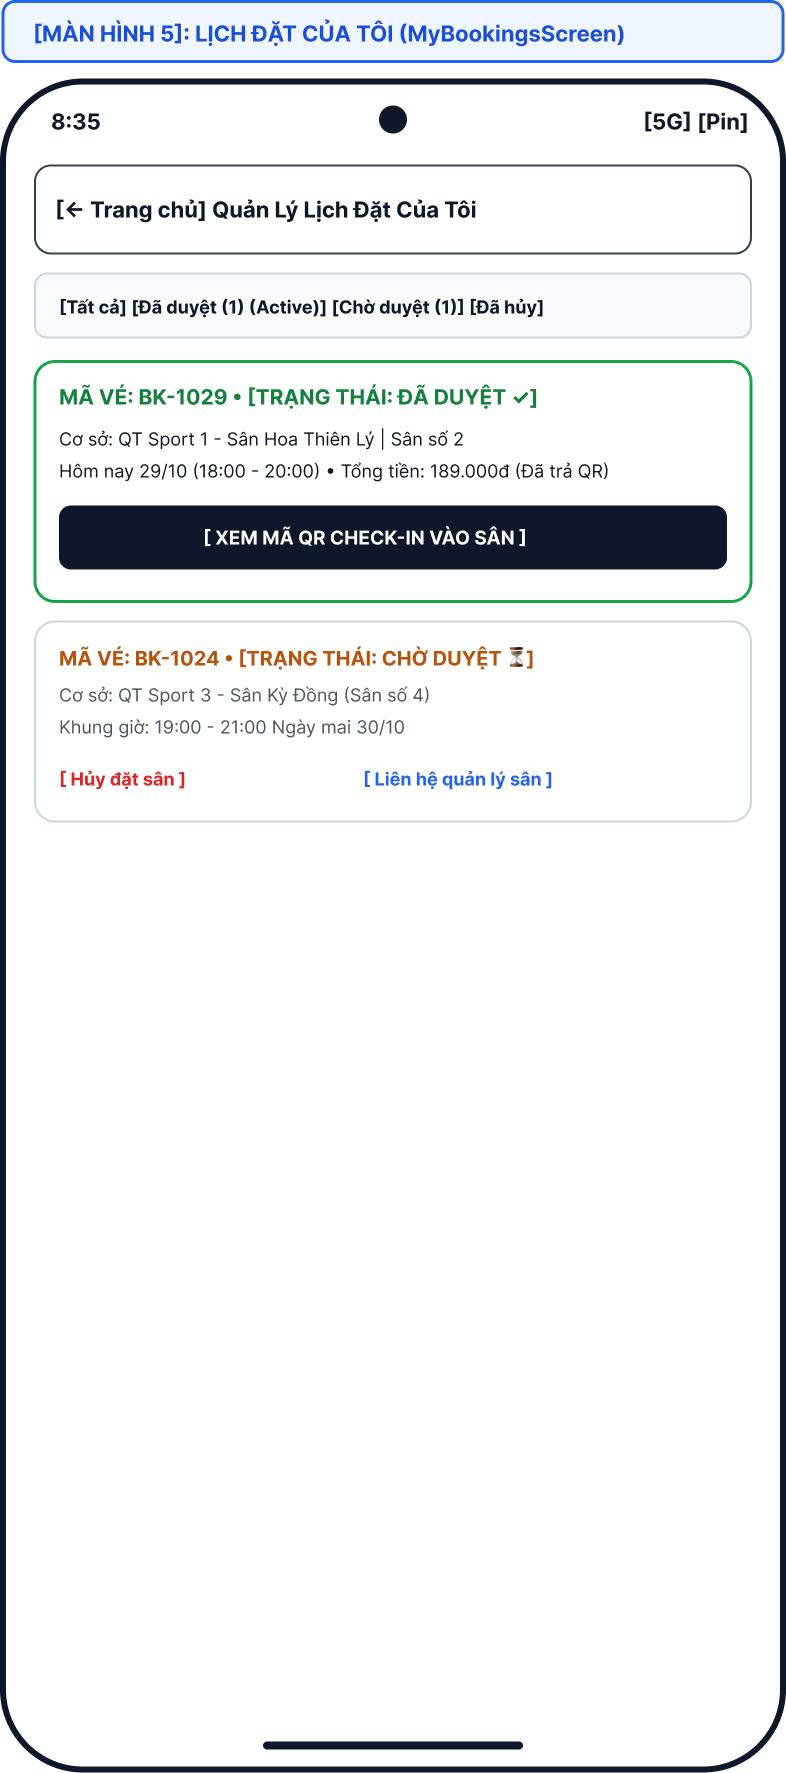
\includegraphics[height=9.5cm, keepaspectratio]{figs/wireframe_quanly.jpg}
\caption{Phác thảo Wireframe sơ bộ giao diện Quản lý lịch đặt sân.}
\label{fig:wf-quanly}
\end{figure}

\textbf{Ở bước 3 (Thiết kế chi tiết và quy chuẩn tương tác):} Tích hợp thanh lọc trạng thái (Tabs Filter: Tất cả, Sắp tới, Lịch sử) và nút tiện ích "Hủy đặt sân" hoặc "Chỉ đường đến sân" qua bản đồ Google Maps.

\textbf{Về kết quả thực hiện thực tế trên hệ thống:} Giao diện thực tế hiển thị danh sách các ca chơi đã đặt với thông tin chi tiết Sân 3 - Cơ sở Hoa Thiên Lý, thời gian 18:00 - 20:00, huy hiệu xác nhận xanh lá và nút tra cứu mã vé điện tử tiện lợi.

\begin{figure}[H]
\centering
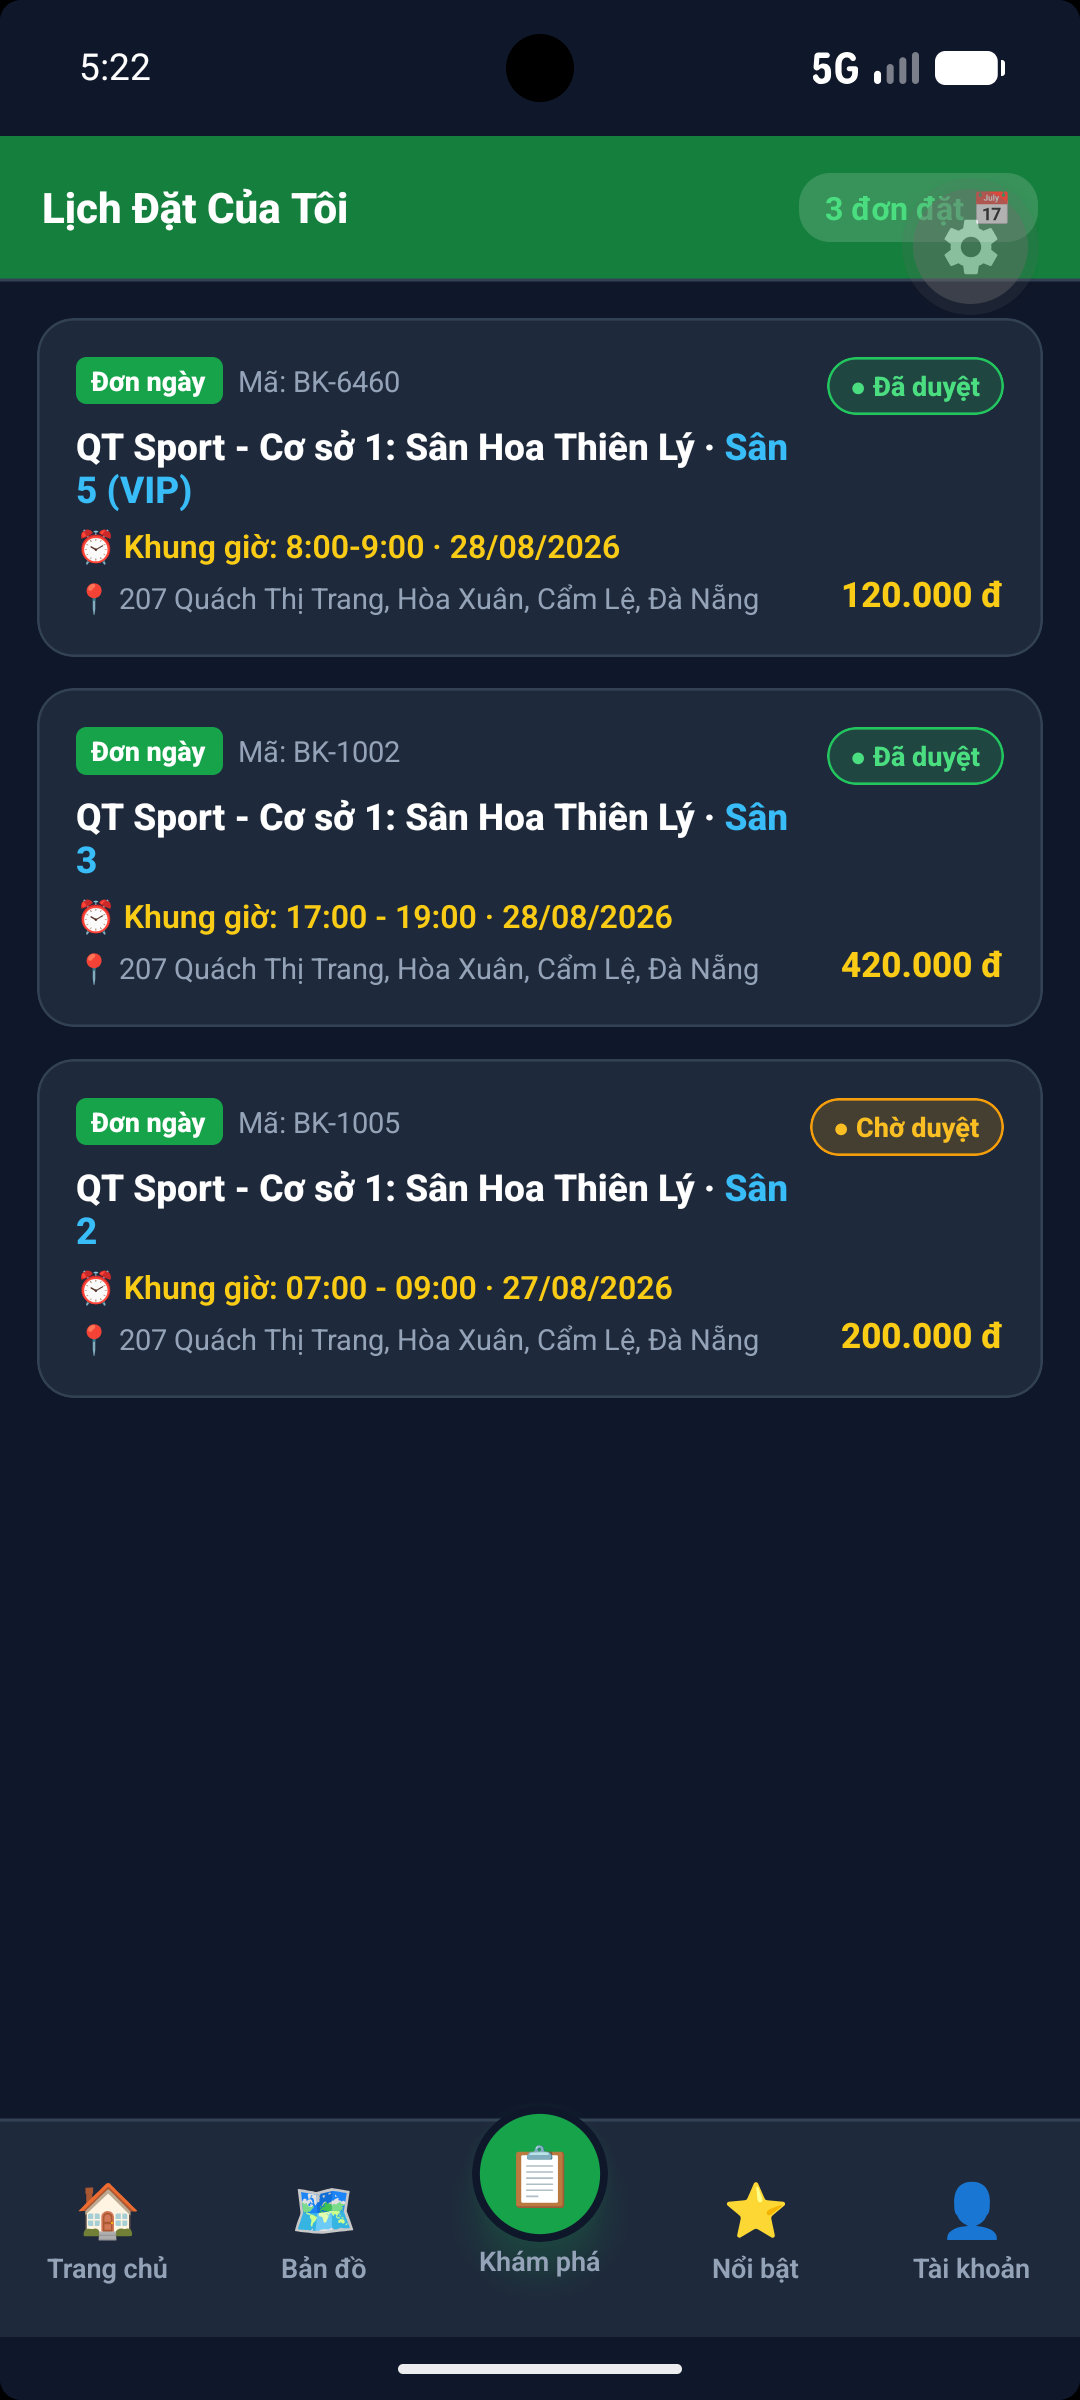
\includegraphics[height=11.5cm, keepaspectratio]{figs/demo_sandadat.png}
\caption{Kết quả thực hiện thực tế giao diện Quản lý lịch đặt sân đã đặt.}
\label{fig:demo-sandadat}
\end{figure}

\section{Dữ liệu (Database)}
\label{sec:database}

\subsection{Giới thiệu tổng quan hệ CSDL quan hệ MySQL}
Hệ thống sử dụng hệ quản trị cơ sở dữ liệu quan hệ \textbf{MySQL 8.0}. Mô hình cơ sở dữ liệu được chuẩn hóa ở dạng chuẩn 3 (Third Normal Form - 3NF) nhằm loại bỏ triệt để hiện tượng trùng lặp dữ liệu, đảm bảo tính nhất quán (Consistency) và toàn vẹn tham chiếu (Referential Integrity) giữa các thực thể cốt lõi trong toàn bộ hệ thống.

\subsection{Thiết kế cấu trúc cơ sở dữ liệu (Sơ đồ ERD \& Data Dictionary)}
Lược đồ quan hệ thực thể (ERD) được thiết kế chi tiết trên MySQL Workbench, bao gồm 8 thực thể quan hệ chặt chẽ với nhau (Hình~\ref{fig:erd-diagram}):

\begin{figure}[H]
\centering
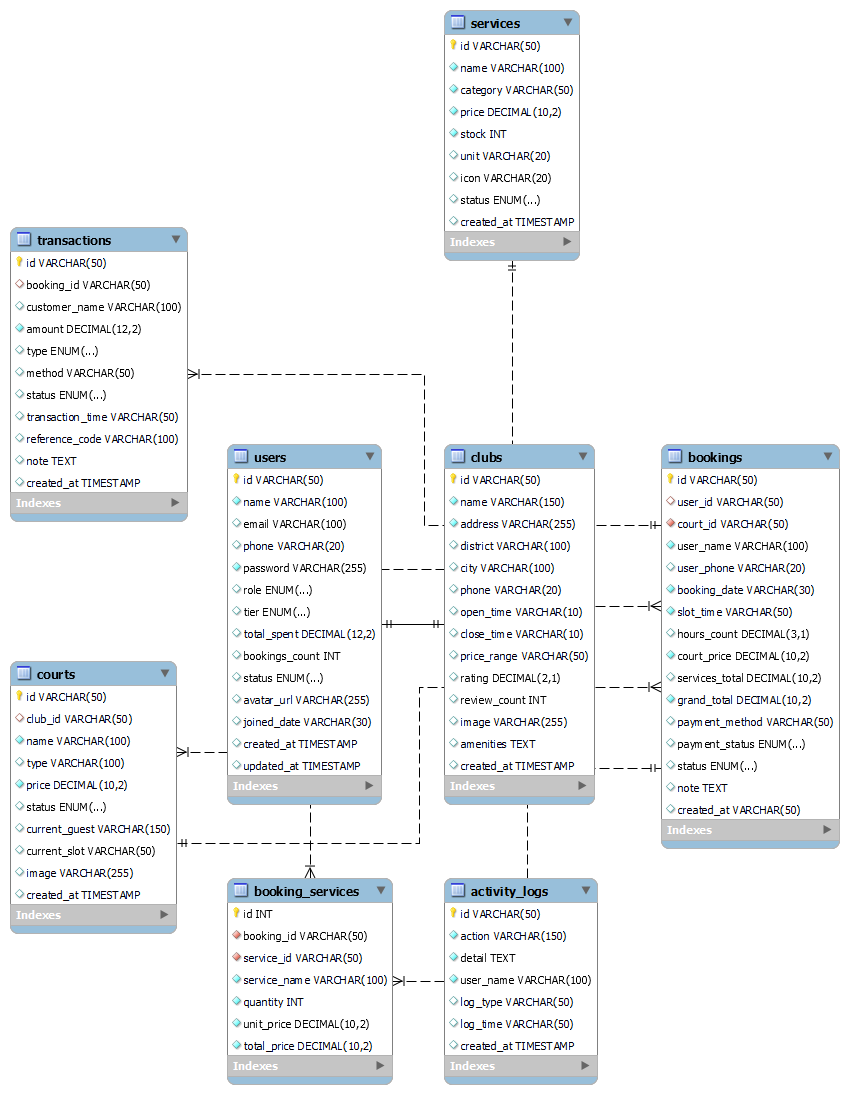
\includegraphics[width=\textwidth]{figs/erd.png}
\caption{Sơ đồ cấu trúc Cơ sở dữ liệu quan hệ (ERD) toàn hệ thống đặt sân.}
\label{fig:erd-diagram}
\end{figure}

Từ điển dữ liệu (Data Dictionary) chi tiết của 6 bảng nòng cốt trong hệ thống được định nghĩa quy chuẩn như sau:

\begin{table}[H]
\centering
\caption{Từ điển dữ liệu bảng users (Tài khoản người dùng).}
\label{tab:dict-users}
\small
\begin{tabular*}{\textwidth}{@{\extracolsep{\fill}}l l l l p{0.35\textwidth}}
\toprule
\textbf{Tên cột} & \textbf{Kiểu dữ liệu} & \textbf{Khóa} & \textbf{Ràng buộc (Constraint)} & \textbf{Diễn giải ý nghĩa} \\
\midrule
id & VARCHAR(50) & PK & PRIMARY KEY, NOT NULL & Mã định danh duy nhất của người dùng \\
name & VARCHAR(100) & -- & NOT NULL & Họ và tên đầy đủ của người dùng \\
email & VARCHAR(100) & -- & UNIQUE, NULL & Địa chỉ thư điện tử người dùng \\
phone & VARCHAR(20) & -- & UNIQUE, NOT NULL & Số điện thoại (tài khoản đăng nhập chính) \\
password & VARCHAR(255) & -- & NOT NULL & Mật khẩu tài khoản (đã băm Bcrypt) \\
role & VARCHAR(20) & -- & DEFAULT 'customer' & Vai trò: 'admin', 'staff', 'customer' \\
tier & VARCHAR(20) & -- & DEFAULT 'Đồng' & Hạng thành viên: Đồng, Bạc, Vàng, Kim Cương \\
\bottomrule
\end{tabular*}
\end{table}

\begin{table}[H]
\centering
\caption{Từ điển dữ liệu bảng clubs (Cụm sân cầu lông / Chi nhánh).}
\label{tab:dict-clubs}
\small
\begin{tabular*}{\textwidth}{@{\extracolsep{\fill}}l l l l p{0.35\textwidth}}
\toprule
\textbf{Tên cột} & \textbf{Kiểu dữ liệu} & \textbf{Khóa} & \textbf{Ràng buộc (Constraint)} & \textbf{Diễn giải ý nghĩa} \\
\midrule
id & VARCHAR(50) & PK & PRIMARY KEY, NOT NULL & Mã định danh duy nhất của cụm sân \\
name & VARCHAR(150) & -- & NOT NULL & Tên thương hiệu cụm sân cầu lông \\
address & VARCHAR(255) & -- & NOT NULL & Địa chỉ thực tế của cơ sở sân \\
district & VARCHAR(100) & -- & NULL & Quận / Huyện đặt cơ sở \\
city & VARCHAR(100) & -- & DEFAULT 'Đà Nẵng' & Thành phố \\
phone & VARCHAR(20) & -- & NULL & Số điện thoại hotline liên hệ bốt trực \\
price\_range & VARCHAR(50) & -- & NULL & Khung giá tham khảo theo giờ \\
\bottomrule
\end{tabular*}
\end{table}

\begin{table}[H]
\centering
\caption{Từ điển dữ liệu bảng courts (Danh mục sân cầu lông).}
\label{tab:dict-courts}
\small
\begin{tabular*}{\textwidth}{@{\extracolsep{\fill}}l l l l p{0.35\textwidth}}
\toprule
\textbf{Tên cột} & \textbf{Kiểu dữ liệu} & \textbf{Khóa} & \textbf{Ràng buộc (Constraint)} & \textbf{Diễn giải ý nghĩa} \\
\midrule
id & VARCHAR(50) & PK & PRIMARY KEY, NOT NULL & Mã định danh duy nhất của sân thi đấu \\
club\_id & VARCHAR(50) & FK & REFERENCES clubs(id) & Mã cụm sân mà sân trực thuộc \\
name & VARCHAR(100) & -- & NOT NULL & Tên sân (Sân 1, Sân 2, Sân VIP...) \\
type & VARCHAR(50) & -- & DEFAULT 'Thảm BWF' & Loại mặt sân (Thảm Yonex BWF, Thảm PVC) \\
price & DECIMAL(10,2) & -- & NOT NULL, DEFAULT 80000 & Đơn giá thuê sân cơ bản trên 1 giờ \\
status & VARCHAR(20) & -- & DEFAULT 'available' & Trạng thái: 'available', 'in\_use', 'maintenance' \\
\bottomrule
\end{tabular*}
\end{table}

\begin{table}[H]
\centering
\caption{Từ điển dữ liệu bảng bookings (Đơn đặt sân).}
\label{tab:dict-bookings}
\small
\begin{tabular*}{\textwidth}{@{\extracolsep{\fill}}l l l l p{0.35\textwidth}}
\toprule
\textbf{Tên cột} & \textbf{Kiểu dữ liệu} & \textbf{Khóa} & \textbf{Ràng buộc (Constraint)} & \textbf{Diễn giải ý nghĩa} \\
\midrule
id & VARCHAR(50) & PK & PRIMARY KEY, NOT NULL & Mã đơn đặt sân duy nhất \\
user\_id & VARCHAR(50) & FK & REFERENCES users(id) & Mã khách hàng thực hiện đặt sân \\
court\_id & VARCHAR(50) & FK & REFERENCES courts(id) & Mã sân được khách hàng lựa chọn thuê \\
booking\_date & VARCHAR(30) & -- & NOT NULL & Ngày đăng ký thi đấu \\
slot\_time & VARCHAR(50) & -- & NOT NULL & Khung giờ thi đấu (ví dụ: '18:00 - 20:00') \\
grand\_total & DECIMAL(10,2) & -- & NOT NULL & Tổng tiền thanh toán cuối cùng \\
payment\_status & VARCHAR(20) & -- & DEFAULT 'paid' & Trạng thái thanh toán: 'paid', 'pending' \\
status & VARCHAR(20) & -- & DEFAULT 'confirmed' & Trạng thái đơn: 'confirmed', 'completed', 'cancelled' \\
\bottomrule
\end{tabular*}
\end{table}

\begin{table}[H]
\centering
\caption{Từ điển dữ liệu bảng services (Danh mục sản phẩm, nước uống \& phụ kiện).}
\label{tab:dict-services}
\small
\begin{tabular*}{\textwidth}{@{\extracolsep{\fill}}l l l l p{0.35\textwidth}}
\toprule
\textbf{Tên cột} & \textbf{Kiểu dữ liệu} & \textbf{Khóa} & \textbf{Ràng buộc (Constraint)} & \textbf{Diễn giải ý nghĩa} \\
\midrule
id & VARCHAR(50) & PK & PRIMARY KEY, NOT NULL & Mã định danh mặt hàng dịch vụ \\
name & VARCHAR(100) & -- & NOT NULL & Tên sản phẩm (Nước khoáng, Cầu lông, Quấn cán) \\
category & VARCHAR(50) & -- & NOT NULL & Phân loại mặt hàng: 'drink', 'shuttlecock', 'gear' \\
price & DECIMAL(10,2) & -- & NOT NULL & Đơn giá bán lẻ tại quầy \\
stock & INT & -- & DEFAULT 0 & Số lượng tồn kho khả dụng \\
\bottomrule
\end{tabular*}
\end{table}

\begin{table}[H]
\centering
\caption{Từ điển dữ liệu bảng booking\_services (Chi tiết dịch vụ đi kèm đơn đặt).}
\label{tab:dict-booking-services}
\small
\begin{tabular*}{\textwidth}{@{\extracolsep{\fill}}l l l l p{0.35\textwidth}}
\toprule
\textbf{Tên cột} & \textbf{Kiểu dữ liệu} & \textbf{Khóa} & \textbf{Ràng buộc (Constraint)} & \textbf{Diễn giải ý nghĩa} \\
\midrule
id & INT AUTO & PK & PRIMARY KEY & Mã bản ghi chi tiết dịch vụ \\
booking\_id & VARCHAR(50) & FK & REFERENCES bookings(id) & Mã đơn đặt sân tương ứng \\
service\_id & VARCHAR(50) & FK & REFERENCES services(id) & Mã dịch vụ / sản phẩm đã mua \\
quantity & INT & -- & NOT NULL, DEFAULT 1 & Số lượng sản phẩm khách hàng yêu cầu \\
total\_price & DECIMAL(10,2) & -- & NOT NULL & Thành tiền (Số lượng $\times$ Đơn giá) \\
\bottomrule
\end{tabular*}
\end{table}

\subsection{Các tập dữ liệu thực nghiệm trong hệ thống}
Dưới đây là các bảng dữ liệu mẫu thực tế đã được nạp (seed data) vào cơ sở dữ liệu MySQL:

\begin{table}[H]
\centering
\caption{Tập dữ liệu thực nghiệm bảng users.}
\label{tab:data-users}
\small
\begin{tabular*}{\textwidth}{@{\extracolsep{\fill}}c l c l c c c}
\toprule
\textbf{id} & \textbf{name} & \textbf{phone} & \textbf{email} & \textbf{role} & \textbf{tier} & \textbf{status} \\
\midrule
u1 & Trần Quốc Trung & 0905591379 & admin@court.vn & \textbf{admin} & Kim Cương & active \\
u2 & Nguyễn Văn An & 0912345678 & an.nguyen@gmail.com & customer & Vàng & active \\
u3 & Lê Thị Bích & 0987654321 & bich.le@gmail.com & customer & Bạc & active \\
u4 & Phạm Quốc Cường & 0933445566 & cuong.pham@gmail.com & customer & Đồng & active \\
u5 & Hoàng Minh Tuấn & 0977889900 & tuan.hoang@court.vn & \textbf{staff} & Đồng & active \\
\bottomrule
\end{tabular*}
\end{table}

\begin{table}[H]
\centering
\caption{Tập dữ liệu thực nghiệm bảng clubs.}
\label{tab:data-clubs}
\small
\begin{tabular*}{\textwidth}{@{\extracolsep{\fill}}c l l c c c c}
\toprule
\textbf{id} & \textbf{name} & \textbf{address} & \textbf{district} & \textbf{city} & \textbf{price\_range} & \textbf{rating} \\
\midrule
c1 & QT Sport - CS 1 (Hoa Thiên Lý) & 207 Quách Thị Trang & Cẩm Lệ & Đà Nẵng & 60-120k/h & 4.9 \\
c2 & QT Sport - CS 2 (Kỳ Đồng) & 93 Kỳ Đồng & Thanh Khê & Đà Nẵng & 50-100k/h & 4.8 \\
c3 & QT Sport - CS 3 (Sơn Trà Pro) & 120 Ngô Quyền & Sơn Trà & Đà Nẵng & 70-130k/h & 5.0 \\
c4 & QT Sport - CS 4 (ECO Center Q7) & 45 Huỳnh Tấn Phát & Quận 7 & TP.HCM & 70-140k/h & 4.9 \\
c5 & QT Sport - CS 5 (Sky Club) & 18D Cộng Hòa & Tân Bình & TP.HCM & 65-130k/h & 4.7 \\
\bottomrule
\end{tabular*}
\end{table}

\begin{table}[H]
\centering
\caption{Tập dữ liệu thực nghiệm bảng courts.}
\label{tab:data-courts}
\small
\begin{tabular*}{\textwidth}{@{\extracolsep{\fill}}c c l l c c c}
\toprule
\textbf{id} & \textbf{club\_id} & \textbf{name} & \textbf{type} & \textbf{price} & \textbf{status} & \textbf{current\_slot} \\
\midrule
1 & c1 & Sân 1 - CS 1 (Hoa Thiên Lý) & Thảm Yonex BWF & 80.000đ & \textbf{available} & -- \\
2 & c1 & Sân 2 - CS 1 (Hoa Thiên Lý) & Thảm Yonex BWF & 80.000đ & \textbf{available} & -- \\
3 & c1 & Sân 3 - CS 1 (Hoa Thiên Lý) & Thảm Yonex BWF & 80.000đ & \textbf{in\_use} & 18:00 - 20:00 \\
5 & c1 & Sân 5 - CS 1 (VIP Thảm Đỏ) & Thảm Victor Pro & 120.000đ & \textbf{available} & -- \\
8 & c1 & Sân 8 - CS 1 (Bảo dưỡng) & Thảm Yonex BWF & 80.000đ & \textbf{maintenance} & Cả ngày \\
\bottomrule
\end{tabular*}
\end{table}

\begin{table}[H]
\centering
\caption{Tập dữ liệu thực nghiệm bảng bookings.}
\label{tab:data-bookings}
\small
\begin{tabular*}{\textwidth}{@{\extracolsep{\fill}}c l c c c c c}
\toprule
\textbf{id} & \textbf{user\_name} & \textbf{court\_id} & \textbf{booking\_date} & \textbf{slot\_time} & \textbf{grand\_total} & \textbf{status} \\
\midrule
bk001 & Nguyễn Văn An & 3 & 12/11/2026 & 18:00 - 20:00 & 160.000đ & \textbf{confirmed} \\
bk002 & Lê Thị Bích & 6 & 12/11/2026 & 17:00 - 19:00 & 180.000đ & \textbf{confirmed} \\
bk003 & Phạm Quốc Cường & 1 & 13/11/2026 & 06:00 - 08:00 & 160.000đ & \textbf{completed} \\
\bottomrule
\end{tabular*}
\end{table}

\begin{table}[H]
\centering
\caption{Tập dữ liệu thực nghiệm bảng services.}
\label{tab:data-services}
\small
\begin{tabular*}{\textwidth}{@{\extracolsep{\fill}}c l c c c c}
\toprule
\textbf{id} & \textbf{name} & \textbf{category} & \textbf{price} & \textbf{unit} & \textbf{stock} \\
\midrule
srv1 & Nước khoáng Aquafina 500ml & drink & 10.000đ & chai & 150 \\
srv2 & Nước bù khoáng Pocari Sweat & drink & 20.000đ & chai & 80 \\
srv3 & Quả cầu lông Hải Yến S90 & shuttlecock & 25.000đ & quả & 200 \\
srv4 & Quấn cán vợt Yonex chính hãng & gear & 35.000đ & cái & 45 \\
\bottomrule
\end{tabular*}
\end{table}
